%%%%%%%%%%%%%%%%%%%%%%%%%%%%%%%%%%%%%%%%%
% The Legrand Orange Book
% LaTeX Template
% Version 2.1.1 (14/2/16)
%
% This template has been downloaded from:
% http://www.LaTeXTemplates.com
%
% Original author:
% Mathias Legrand (legrand.mathias@gmail.com) with modifications by:
% Vel (vel@latextemplates.com)
%
% License:
% CC BY-NC-SA 3.0 (http://creativecommons.org/licenses/by-nc-sa/3.0/)
%
% Compiling this template:
% This template uses biber for its bibliography and makeindex for its index.
% When you first open the template, compile it from the command line with the 
% commands below to make sure your LaTeX distribution is configured correctly:
%
% 1) pdflatex main
% 2) makeindex main.idx -s StyleInd.ist
% 3) biber main
% 4) pdflatex main x 2
%
% After this, when you wish to update the bibliography/index use the appropriate
% command above and make sure to compile with pdflatex several times 
% afterwards to propagate your changes to the document.
%
% This template also uses a number of packages which may need to be
% updated to the newest versions for the template to compile. It is strongly
% recommended you update your LaTeX distribution if you have any
% compilation errors.
%
% Important note:
% Chapter heading images should have a 2:1 width:height ratio,
% e.g. 920px width and 460px height.
%
%%%%%%%%%%%%%%%%%%%%%%%%%%%%%%%%%%%%%%%%%

%----------------------------------------------------------------------------------------
%	PACKAGES AND OTHER DOCUMENT CONFIGURATIONS
%----------------------------------------------------------------------------------------

\documentclass[11pt,fleqn]{book} % Default font size and left-justified equations

\usepackage{wasysym}
\usepackage{esint} % various fancy integral symbols
\usepackage{tikz}
\usepackage{tikz-3dplot}
\usepackage{pgfplots}
\usepackage[french]{babel}
\pgfplotsset{compat=1.17}

\usetikzlibrary {arrows.meta} 

\newcommand{\dd}{\mathrm{d}}
\newcommand{\div}{\mathrm{div}}
\newcommand{\rot}{\vv{\mathrm{div}}}
\newcommand{\grad}{\vv{\mathrm{grad}}}

\usepackage[d]{esvect}

\definecolor{myred}{RGB}{243,102,25}
%----------------------------------------------------------------------------------------

\input{structure} % Insert the commands.tex file which contains the majority of the structure behind the template

\begin{document}
%----------------------------------------------------------------------------------------
%	TITLE PAGE
%----------------------------------------------------------------------------------------

%\begingroup
%\thispagestyle{empty}
%\begin{tikzpicture}[remember picture,overlay]
%\coordinate [below=12cm] (midpoint) at (current page.north);
%\node at (current page.north west)
%{\begin{tikzpicture}[remember picture,overlay]
%\node[anchor=north west,inner sep=0pt] at (0,0) {
\includegraphics[width=\paperwidth]{background}}; % Background image
%\draw[anchor=north] (midpoint) node [fill=ocre!30!white,fill opacity=0.6,text opacity=1,inner sep=1cm]{\Huge\centering\bfseries\sffamily\parbox[c][][t]{\paperwidth}{\centering Cours de Physique-Chimie\\[15pt] % Book title
%{}\\[20pt] % Subtitle
%{\huge Lycée Baimbridge MP 2025-2026}}}; % Author name
%\end{tikzpicture}};
%\end{tikzpicture}
%\vfill
%\endgroup

%----------------------------------------------------------------------------------------
%	COPYRIGHT PAGE
%----------------------------------------------------------------------------------------

%\newpage
%~\vfill
%\thispagestyle{empty}

%\noindent Copyright \copyright\ CC BY 4.0 2025 Basile Poujol\\ % Copyright notice

%\noindent Licensed under the Creative Commons Attribution-NonCommercial 4.0 Unported License (the ``License''). You may not use this file except in compliance with the License. You may obtain a copy of the License at \url{http://creativecommons.org/licenses/by-nc/3.0}. See the License for the specific language governing permissions and limitations under the License.\\ % License information

%----------------------------------------------------------------------------------------
%	TABLE OF CONTENTS
%----------------------------------------------------------------------------------------

%\usechapterimagefalse % If you don't want to include a chapter image, use this to toggle images off - it can be enabled later with \usechapterimagetrue

\chapterimage{orage.jpg} % Table of contents heading image

%\pagestyle{empty} % No headers

%\tableofcontents % Print the table of contents itself

%\cleardoublepage % Forces the first chapter to start on an odd page so it's on the right

%\pagestyle{fancy} % Print headers again



%\part{\'{E}lectromagnétisme}

\setcounter{chapter}{2}

\chapter{\'{E}lectrostatique}

\paragraph{Introduction}

L'électrostatique est la branche de la physique qui s'intéresse à la présence de charges électriques en certains points de l'espace, et leurs effets physiques.

L'électrostatique ne s'intéresse pas aux déplacements des charges électriques et donc aux courants électriques. En ce sens, une grande partie de l'électronique ne rentre pas dans le cadre de l'électrostatique.

Les interactions électrostatiques jouent un rôle très important à l'échelle microscopique : ce sont elles qui maintiennent la cohésion des atomes et conduisent à la formation de molécules ou de solides cristallins. Elles peuvent aussi occasionnellement se manifester à l'échelle macroscopique, par exemple dans un condensateur ou dans un orage.

Dans ce chapitre, nous allons proposer une description des charges électriques ponctuelles, valable à l'échelle microscopique, puis une description continue plus adaptée à l'échelle macroscopique. Dans le cours et le TD, nous expliquerons des phénomènes physiques tels que la foudre, la solvatation des ions ou encore le fonctionnement d'un condensateur.

\section{Champ électrique}

\subsection{La charge électrique}

\begin{definition}[Charge électrique]
La charge électrique est une propriété fondamentale de la matière. Elle se mesure en Coulomb (C) est quantifiée par la charge élémentaire $e = 1.6 \times 10^{-19} C$.
\end{definition}

La charge électrique est portée par des porteurs élémentaires: les protons (charge $+e$) et les électrons (charge $-e$). Quelques exemples:
\begin{itemize}
    \item Les molécules sont neutres électriquement (autant de protons que d'électrons);
    \item Dans les métaux, les électrons se déplacent librement et permettent la propagation de courant électrique;
    \item Les ions constituent des porteurs de charge fixes dans les solides cristallins;
    \item En solution aqueuse, les ions peuvent se déplacer et ainsi permettre la circulation de courant électrique.
\end{itemize}

\begin{figure}[h]
\centering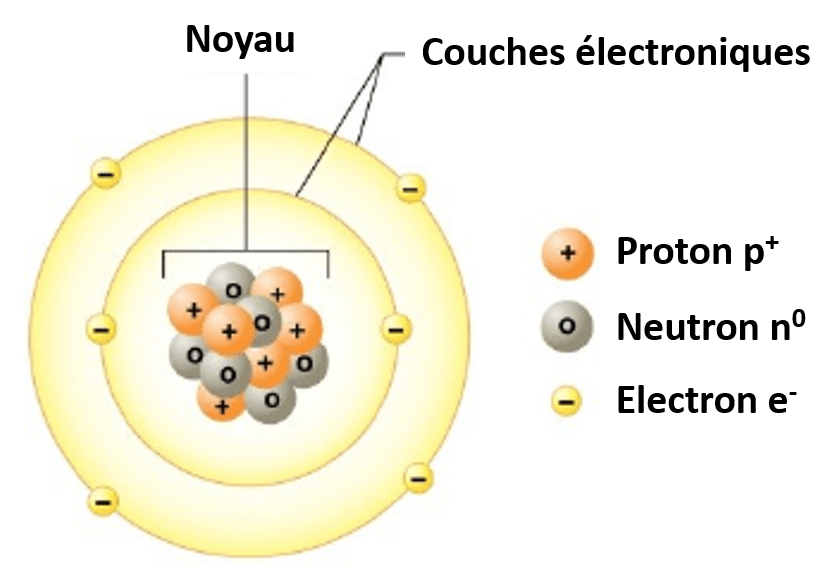
\includegraphics[height=0.27\textwidth]{Pictures/charges_atome.png} 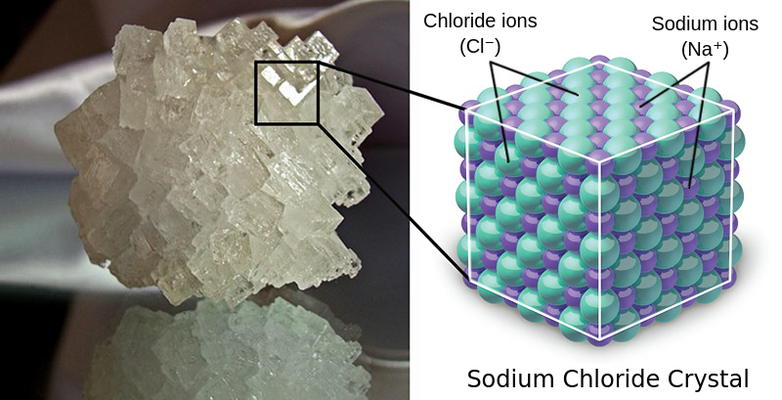
\includegraphics[height=0.27\textwidth]{Pictures/ions_cristal.png}
\caption{Importance des interactions électrostatiques dans la nature. A gauche : vision classique de la structure interne de l'atome (source biologie101.fr). A droite : les interactions électrostatiques entre les ions sont responsables de la structure cristalline cubique du sel (source theory.labster.com) }
\end{figure}

\subsection{Force électrostatique}

\begin{theorem}[Loi de Coulomb]
Une charge $q_1$ localisée en $M_1$ exerce sur une charge $q_2$ localisée en $M_2$ une force électrostatique: 
\begin{equation}
    \vv F_{1 \rightarrow 2} = \frac{q_1 q_2}{4 \pi \varepsilon_0 r^2} \vv{e_r}
\end{equation}
où l'on a défini $r = \left\lVert \vv{M_1 M_2} \right\lVert$ et $\vv{e_r} = \frac{\vv{M_1 M_2}}{\left\lVert \vv{M_1 M_2} \right\lVert}$.\\
La force est \textbf{répulsive} si les charges sont de même signe et \textbf{attractive} sinon.
\end{theorem}

\begin{figure}[htbp]
\centering
\begin{tikzpicture}

\filldraw[black] (0,0) circle (2pt) node[anchor=west]{$M_1$};
\filldraw[black] (2,1) circle (2pt) node[anchor=east]{$M_2$};
\draw[-{Classical TikZ Rightarrow},thick] (2,1) -- (2.5,1.25) node[anchor=west]{$\vv F_{1 \rightarrow 2}$};
\draw[-{Classical TikZ Rightarrow},thick] (0,0) -- (-.5,-.25) node[anchor=east]{$\vv F_{2 \rightarrow 1}$};
\filldraw[black] (1,-1) circle (0pt) node[anchor=north]{$q_1>0\,;\,q_2>0$};

\filldraw[black] (5,0) circle (2pt) node[anchor=east]{$M_1$};
\filldraw[black] (7,1) circle (2pt) node[anchor=west]{$M_2$};
\draw[-{Classical TikZ Rightarrow},thick] (7,1) -- (6.5,0.75) node[anchor=south east]{$\vv F_{1 \rightarrow 2}$};
\draw[-{Classical TikZ Rightarrow},thick] (5,0) -- (5.5,.25) node[anchor=north west]{$\vv F_{2 \rightarrow 1}$};
\filldraw[black] (6,-1) circle (0pt) node[anchor=north]{$q_1>0\,;\,q_2<0$};

\end{tikzpicture}
\caption{La force de Coulomb, pour des charges de même signe et de signe opposé.}
\end{figure}

\begin{remark}
    La force de Coulomb a été découverte expérimentalement et n'a pas de fondement théorique : il s'agit d'une loi empirique. Cette force est formellement analogue à la force gravitationnelle. Ainsi, on constatera de nombreuses similarités entre ce chapitre d'électrostatique et les propriétés de la gravitation en mécanique classique.
\end{remark}

\begin{encart}[L'expérience de Coulomb]

Après avoir passé 8 ans comme ingénieur en Martinique, Coulomb s'installe à Paris pour mener des recherches et réalise de nombreuses expériences. En particulier, il met au point la \textit{balance de Coulomb}, qui fonctionne à l'aide du phénomène de torsion d'un fil. Comme vu en MPSI, un fil tordu d'un angle $\theta$ exerce à ses extrémités un couple proportionnel à cet angle $\Gamma = C \theta$.

\begin{center}
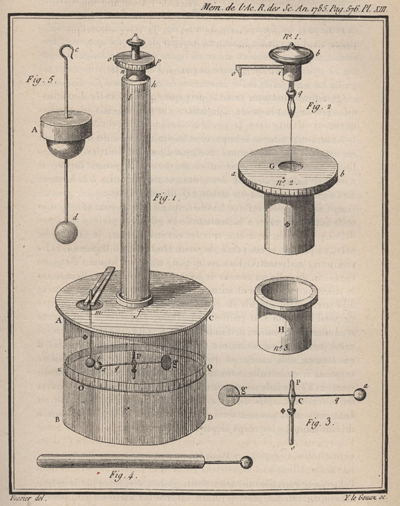
\includegraphics[width=0.3\textwidth]{Pictures/balance_coulomb.jpg} \hspace{0.1\textwidth}
\begin{tikzpicture}

\filldraw[black] (0,0) circle (2pt) node[anchor=west]{$q_1$};
\filldraw[black] (0.228,1.147) circle (2pt) node[anchor=west]{$\,q_2$};
\filldraw[black] (3,0) circle (1.5pt) node[anchor=south west]{$\,\,O$};
\draw[-,thick] (0.228,1.147) -- (2.82,0.06) node[midway,anchor=south]{$R$};
\draw[thick,dashed] (0,0) arc (180:240:3);
\draw[thick,dashed] (0,0) arc (180:120:3);
\draw[thick] (3.2,0) arc (0:360:0.2);
\draw[thick,<->] (-0.3,0) arc (180:157.5:3.3) node[midway,anchor=east]{$d$};
\draw[->,thick] (0.228,1.147) -- (0.456,2.29) node[anchor=south east]{$\vv F_{1 \rightarrow 2}$};
\draw[thick,<-] (3.65,0) arc (360:157.5:0.65) node[midway,anchor=north]{$\Gamma = -C \theta$} ;

\end{tikzpicture}
\end{center}

Ce phénomène est utilisé dans la balance de Coulomb: deux charges sont mises en contact et l'une d'entre elles est attaché à une barre en rotation libre autour de l'axe du fil. On note $R$ la distance entre le fil et la boule. A l'équilibre, le couple de torsion du fil s'équilibre avec le couple de la force électrostatique:
\begin{equation}
    C \theta = \frac{q_1 q_2}{4 \pi \varepsilon_0 d^2} R
\end{equation}
Coulomb affirme avoir, dans ses expériences, obtenu un angle $\theta$ qui varie proportionellement à $1/d^2$. Ce résultat a été mis en doute par la communauté, car dans son article original Coulomb a très peu décrit son expérience et personne n'a réussi à reproduire ses résultats avec ce dispositif (y compris avec les techniques modernes). Ceci pourrait être dû à la présence de fuites électriques, et plusieurs articles scientifiques suggèrent que Coulomb a peut-être sélectionné les résultats qui confirmaient le mieux sa prédiction théorique. Quoi qu'il en soit, si à l'époque l'idée que deux corps puissent exercer une force l'un sur l'autre sans se toucher était très mal accueillie, l'intuition de Coulomb était effectivement la bonne et la loi a depuis été démontrée par d'autres dispositifs.
    
\end{encart}

\begin{encart}[Quelques ordres de grandeur]

La charge élémentaire vaut $e = 1,6 \times 10^{-19}$\,C. La permittivité diélectrique du vide, $\varepsilon_0$, est une constante physique fondamentale. Elle caractérise l'intensité des interactions électriques dans le vide. 

La force électrostatique est beaucoup plus intense que la force gravitationnelle. Supposons par exemple que vous vous trouvez à environ $d=1$\,m d'une autre personne. En supposant que vous pesez $m_1 = m_2 = 65$\,kg, la force gravitationnelle qui vous attire l'un l'autre est donnée par :
\begin{equation}
    || \vv F_{grav} || = \mathcal{G} \frac{m_1 m_2}{d^2} \approx 3 \times 10^{-7} N
\end{equation}
ce qui correspond au poids d'un objet de masse $\mu = || \vv F_{grav} ||/g = 10^{-8}$\,kg, c'est-à-dire le poids d'une dizaine de grains de sable. La force gravitationnelle est très faible et n'est généralement ressentie que lorsqu'au moins l'un des deux corps concernés a une masse très importante.

Intéressons nous maintenant aux ordres de grandeur de la force électrostatique. En supposant que vous êtes constitués d'eau, la masse molaire de l'eau étant de  $M_{H_2 O} =18$\,g$\cdot$mol$^{-1}$, vous contenez environ un nombre de molécules d'eau égal à :
\begin{equation}
    N = \frac{\mathcal{N}_A m_1}{M_{H_2 O}} \approx 2 \times 10^{27}
\end{equation}
En supposant que vous donniez les électrons de 1\% de vos molécules d'eau à votre voisin, vous allez perdre une charge totale égale à :
\begin{equation}
    q = \frac{1}{100} N e \approx 3 \times 10^6 \mathrm{C}
\end{equation}
Votre voisin sera alors chargé de la charge opposée $-q$. La force électrostatique qui vous attirera sera alors :
\begin{equation}
    || \vv F_{elec} || =  \frac{q^2}{4 \pi \varepsilon_0 d^2} \approx 8 \times 10^{22} N
\end{equation}
Ceci correspond au poids d'un objet de masse $\mu = || \vv F_{elec} ||/g \approx 10^{22}$\,kg, soit environ la masse de Pluton !

Autrement dit, la force électrostatique est une force extrêmement intense ! Elle a tendance à rassembler les charges positives et négatives sur des distances très courtes, et à créer des ensembles électriquement neutres. C'est en particulier la force électrostatique qui maintient les électrons autour des atomes, qui explique la structure des cristaux et leur solidité, et plus généralement qui est responsable de la cohésion des solides et des liquides. 

La force de gravitation est beaucoup plus faible et n'a une importance que pour les objets massifs qui sont électriquement neutres.
\end{encart}

\subsection{Champ électrique}

De manière analogue à la gravitation, l'existence d'une interaction à distance entre deux corps chargés électriquement se traduit par l'existence d'un champ de vecteurs :

\begin{definition}[Champ électrique]
    Le champ électrique, noté $\vv E$, indique en tout point la force électrostatique subie par une particule ponctuelle immobile de charge unité. Il se mesure en Volts-mètres (V$\cdot$m). Une particule de charge $q$ se trouvant dans un champ électrique $\vv E$ subit alors une force électrostatique $\vv F = q \vv E$. 
\end{definition}

\begin{remark}
    Rappel de MPSI : dans le cas où la particule est en mouvement et soumise à un champ magnétique, elle subit également une force magnétique $\vv F_{mag} = q \vv v \wedge \vv B$. La somme de la force électrique et magnétique correspond à la \textbf{force de Lorentz}:
    \begin{equation}
        \vv F = q ( \vv E + \vv v \wedge \vv B )
    \end{equation}
\end{remark}

Pourquoi définir le champ électrique ? Il nous permet de décrire la force subie par une particule chargée sans avoir besoin de connaître la position de toutes les charges électriques positives et négatives situées autour de la particule qui nous intéresse.

Le champ électrique est un outil particulièrement utile en raison de sa propriété d'additivité : la force électrostatique est linéaire en fonction de la charge qui exerce cette force. Ainsi, le champ électrique produit par une particule est proportionnel à la charge de cette particule. Cette propriété se généralise au cas où deux particules produisant le champ électrique sont placées à des endroits différents\,:

\begin{proposition}[Principe de superposition pour des charges ponctuelles]
    Soient deux particules chargées $M_1$ et $M_2$, produisant respectivement des champs électriques $\vv E_1$ et $\vv E_2$. Le champ électrique produit par l'ensemble des deux particules $\{ M_1,M_2\}$ est $\vv E_1 + \vv E_2$.
\end{proposition}

De manière analogue au champ gravitationnel, nous définissons les lignes de champ :

\begin{definition}[Lignes de champ]
    Une ligne de champ électrique est une ligne parallèle en tout point au vecteur champ électrique $\vv E$. Les lignes de champ sont orientées dans le sens du champ électrique.
\end{definition}

\begin{example}[Lignes de champ produites par une charge ponctuelle]
    Considérons le champ électrique produit par une charge ponctuelle $q$. On se place dans le système de coordonnées polaires ayant pour origine l'emplacement de la charge ponctuelle. Le champ électrique s'écrit, en utilisant la forme de la force électrostatique:
    \begin{equation}
        \vv E = \frac{q}{4 \pi \varepsilon_0 r^2} \vv{e_r}
    \end{equation}
    En tout point de l'espace, $\vv E$ est colinéaire au vecteur unitaire $\vv{e_r}$, ainsi les lignes de champ sont des demi-droites partant de l'origine et orientées vers l'extérieur.
\end{example}

\begin{figure}[htbp]
    \centering
    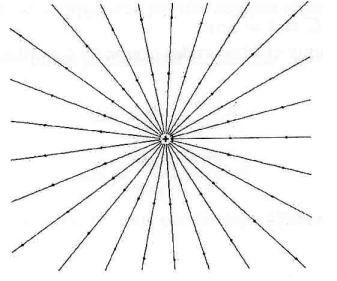
\includegraphics[height=0.33\linewidth]{Pictures/lignes_de_champ_1charge.png}
    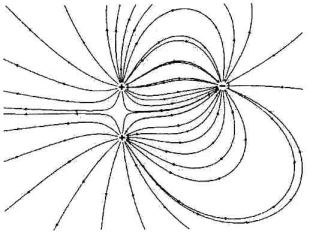
\includegraphics[height=0.33\linewidth]{Pictures/lignes_de_champ_3charges.png}
    \caption{Lignes de champ produites par une charge ponctuelle (à gauche) et par 3 charges ponctuelles (à droite). Les lignes partent des charges positives et se terminent sur les charges négatives. Source : université de technologie de Compiègne.}
\end{figure}

\subsection{Potentiel électrique}

Calculons le travail de la force électrique le long de la trajectoire d'une particule chargée. Soit une particule ponctuelle chargée d'une charge $q$ et parcourant un chemin infinitésimal $\vv{\dd \ell}$.  Le travail élémentaire exercé par la force électrique sur la particule le long de ce déplacement est donné par:
\begin{equation}
    \delta W = \vv F \cdot \vv{\dd \ell} = q \vv E \cdot \vv{\dd \ell}
\end{equation}
si bien que le travail de la force le long d'un chemin macroscopique $\Gamma$ reliant deux points $A$ et $B$ s'écrit:
\begin{equation}
    W = \int_\Gamma q \vv E \cdot \vv{\dd \ell}
\end{equation}

Cette intégrale correspond à ce que l'on nomme la circulation du champ électrique :

\begin{definition}
    La circulation du champ électrostatique $\vv E$ le long d'un chemin $\Gamma$ correspond à l'intégrale du champ électrique le long de ce chemin :
    \begin{equation}
        \mathcal{C} = \int_\Gamma \vv E \cdot \vv{\dd \ell}
    \end{equation}
\end{definition}

\begin{example}
    Calculons le travail issu du déplacement d'une particule $M$ de charge $q$ au voisinage d'une particule charge $q_0$ située sur l'origine. La particule $M$ est soumise à la force électrostatique de Coulomb et on a:
    \begin{align}
        W &= \int_\Gamma q \vv E \cdot \vv{\dd \ell} \\
        &= \int_\Gamma \frac{q q_0}{4 \pi \varepsilon_0 r^2} \vv{e_r} \cdot \vv{\dd \ell}\\
        &=  \frac{q q_0}{4 \pi \varepsilon_0} \int_\Gamma \frac{\mathrm{d}r}{r^2} \\
        &= \frac{q q_0}{4 \pi \varepsilon_0} \left(\frac{1}{r_A} - \frac{1}{r_B} \right)
    \end{align}
\end{example}
On constate que le travail de la force électrostatique ne dépend que de la position initiale et de la position finale de la particule: il est indépendant du chemin suivi. Nous avons vu cela pour une charge ponctuelle, mais le résultat se généralise à tout champ électrique produit par un ensemble de charges:

\begin{proposition}[Conservativité de la force électrique]
    La force électrostatique est une force \textbf{conservative}.
\end{proposition}

Dans le cas d'une seule particule chargée, la force électrique dérive d'un potentiel, en effet il est possible d'écrire son travail comme une différence d'énergie potentielle électrique :
\begin{equation}
    W = - \Delta E_{pot} =  E_{pot,A} - E_{pot,B}
\end{equation}
avec
\begin{equation}
    E_{pot} = \frac{q q_0}{4 \pi \varepsilon_0 r} + C
\end{equation}
$C$ est une constante que l'on prend généralement égale à zéro afin d'avoir une énergie potentielle électrique nulle en l'absence d'interaction avec d'autres charges ($r \to \infty$).

\begin{definition}[Potentiel électrique]
    On définit le potentiel électrostatique $V(M)$ comme l'énergie potentielle électrostatique qu'aurait une charge unité si elle était placée au point $M$.
    
    L'énergie électrostatique d'une particule de charge $q$ s'écrit alors:
    \begin{equation}
        E_{pot} = q V
    \end{equation}
    Le potentiel électrostatique se mesure en Volts (V).
\end{definition}

Pour visualiser le potentiel électrique, on dessine souvent des surfaces équipotentielles (ou lignes équipotentielles si le problème est à deux dimensions):
\begin{definition}
    Une surface équipotentielle est une surface sur laquelle le potentiel électrique a une valeur constante.
\end{definition}

\begin{proposition}
    Le champ électrique est opposé au gradient du potentiel électrique:
    \begin{equation}
    \vv E = -\vv{\mathrm{grad}}(V)
    \end{equation}
\end{proposition}

\begin{demonstration}
Le travail élémentaire de la force électrique le long d'un chemin $\vv{\dd \ell}$ peut s'écrire d'une part:
\begin{equation}
    \delta W = \vv E \cdot \vv{\dd \ell}
\end{equation}
et d'autre part:
\begin{equation}
    \delta W = -\mathrm{d}E_{pot} = - q \mathrm{d} V = - q\,\vv{\mathrm{grad}}(V) \cdot \vv{\dd \ell}
\end{equation}
par propriété de l'opérateur gradient. Par identification, on en déduit:
\begin{equation}
    \vv E \cdot \vv{\dd \ell} = -\vv{\mathrm{grad}}(V) \cdot \vv{\dd \ell}
\end{equation}
Ceci étant vrai pour tout élément $\vv{\dd \ell}$ on en déduit que:
\begin{equation}
    \vv E = -\vv{\mathrm{grad}}(V)
\end{equation}
\end{demonstration}

De la même manière que pour le champ gravitationnel, cette relation implique les propriétés géométriques suivantes :
\begin{proposition}
    Les surfaces équipotentielles et les lignes de champ sont orthogonales.
\end{proposition}

\begin{proposition}
    L'intensité du champ électrique est inversement proportionnelle à la distance entre les équipotentielles.
\end{proposition}

A travers la lecture d'une carte de lignes équipotentielles, on peut donc retrouver la direction et l'intensité du champ électrique en tout point de l'espace.

\begin{figure}[htbp]
    \centering
    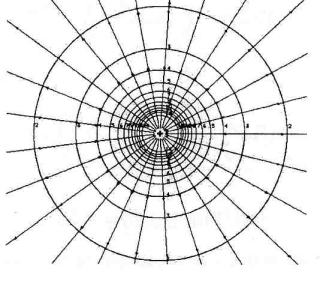
\includegraphics[height=0.33\linewidth]{Pictures/equipotentielles_1charge.png}
    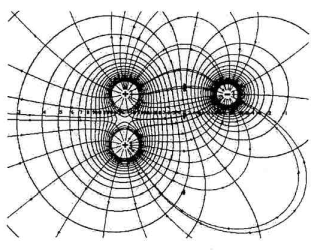
\includegraphics[height=0.33\linewidth]{Pictures/equipotentielles_3charges.png}
    \caption{Lignes de champ et équipotentielles produites par une charge ponctuelle (à gauche) et par 3 charges ponctuelles (à droite). Les équipotentielles sont perpendiculaires aux lignes de champ. Source : université de technologie de Compiègne.}
\end{figure}

Pour une charge ponctuelle, le potentiel électrique $V$ ne dépend que du rayon $r$, les équipotentielles sont donc des sphères centrées sur la charge concernée. Le champ électrique étant plus fort au voisinage de la charge, les équipotentielles y sont plus rapprochées.


%Généralisation à une situation quelconque:
%En l'absence d'induction, le rotationnel du champ électrique est nul:
%\begin{equation}
%    \vv{\mathrm{rot}}(\vv E) = - \frac{\partial \vv B}{\partial t} = \vv 0
%\end{equation}
%On en déduit que le champ électrique peut s'écrire comme le gradient d'un potentiel électrique:
%\begin{equation}
%    \exists V, \vv E = -\vv{\mathrm{grad}}(V)
%\end{equation}
%La force électrostatique dérive donc d'un potentiel quelle que soit la forme de la source de champ électrique, et la force électrique est bien une force conservative.

\begin{encart}[Analogie entre potentiel électrostatique et topographie]
    La carte topographique fournit une bonne analogie pour les équipotentielles et les lignes de champ. En effet, l'énergie potentielle de pesanteur s'écrit, pour une masse $m$ :
    \begin{equation}
        E_p = m g z
    \end{equation}
    si bien que les isolignes d'altitude correspondent aux équipotentielles. Les "lignes de champ" correspondent à la trajectoire d'une particule libre soumise au champ de pesanteur. Elles sont matérialisées par le tracé des cours d'eau. On constate sur les cartes topographiques que les cours d'eau sont toujours orientés perpendiculairement aux isolignes, de la même manière qu'en électrostatique les équipotentielles sont perpendiculaires aux lignes du champ électrique. On le voit très bien sur la carte suivante de la montagne de la Capesterre (source Géoportail). Les isolignes (équipotentielles) sont en marron, et le réseau hydrographique (lignes de champ) est en bleu :\\
    
    \centering 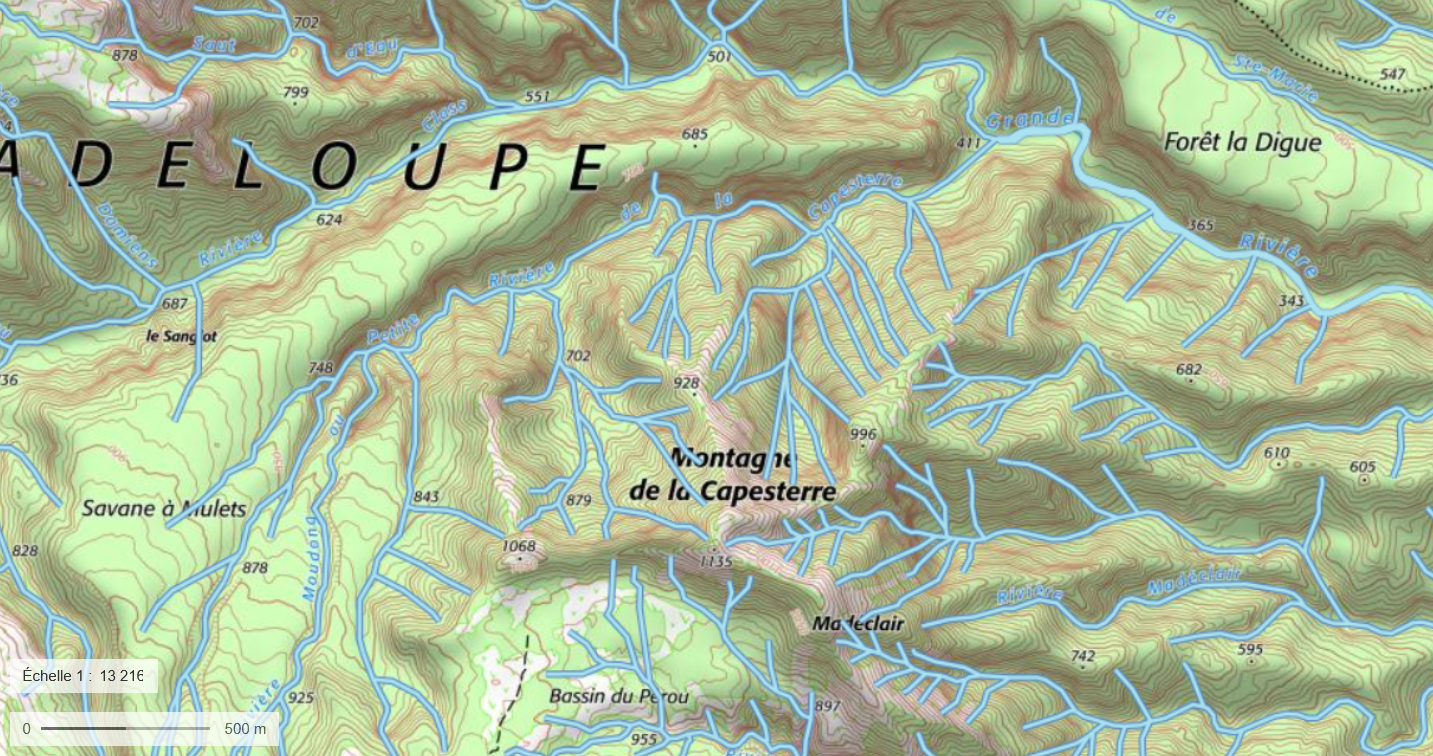
\includegraphics[width=0.9\textwidth]{Pictures/isolignes.png}

    De la même manière que l'on peut orienter les lignes de champ en électrostatique mais pas les équipotentielles, on peut orienter le tracé des cours d'eau sur une carte, mais pas les isolignes.
\end{encart}


Une conséquence importante de cette propriété est l'effet de pointe. Si une pointe se trouve dans un champ électrique donné, elle va dévier et resserrer les équipotentielles à son voisinage, créant ainsi un champ électrique plus intense au voisinage de la pointe, comme cela est visible sur la figure \ref{fig:effet_pointe}.


\begin{encart}[L'effet de pointe et l'arbre à fèves Tonka]
    Une étude publiée en mai 2025, et menée dans un institut de recherche tropical à Panama par Evan Gora, Helene Muller-Landau et Katherine Cushman et leurs collègues internationaux, a montré que l'effet de pointe est aussi utilisé dans la forêt tropicale par l'arbre à fève Tonka. Il est résistant à la foudre et est également plus haut que les autres. Via l'effet de pointe, il renforce le champ électrique autour de lui et augmente sa probabilité d'être frappé par un éclair. Ceci lui permet de tuer les lianes qui l'infestent et ses voisins (qui ne sont pas résistants à la foudre) et favorise son développement. Les scientifiques suggèrent que la résistance de l'arbre aux éclairs pourrait être due à une résistance électrique $R$ de l'arbre plus faible. Etant donné que la puissance dissipée par le passage d'un éclair d'une intensité $I$ est donnée par $\mathcal{P} = R I^2$, une résistance plus faible permettrait donc de limiter le dégagement de chaleur par effet Joule et d'empêcher la combustion de l'arbre.

{\small Référence de l'article scientifique : Gora, Evan M., et al. "How some tropical trees benefit from being struck by lightning: evidence for Dipteryx oleifera and other large‐statured trees." New Phytologist 246.4 (2025): 1554-1566.}
 \end{encart}
 
 
\begin{figure}[htbp]
    \centering
    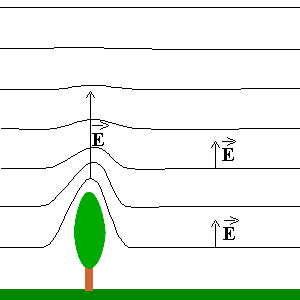
\includegraphics[width=0.49\linewidth]{Pictures/effet_de_pointe.png}
    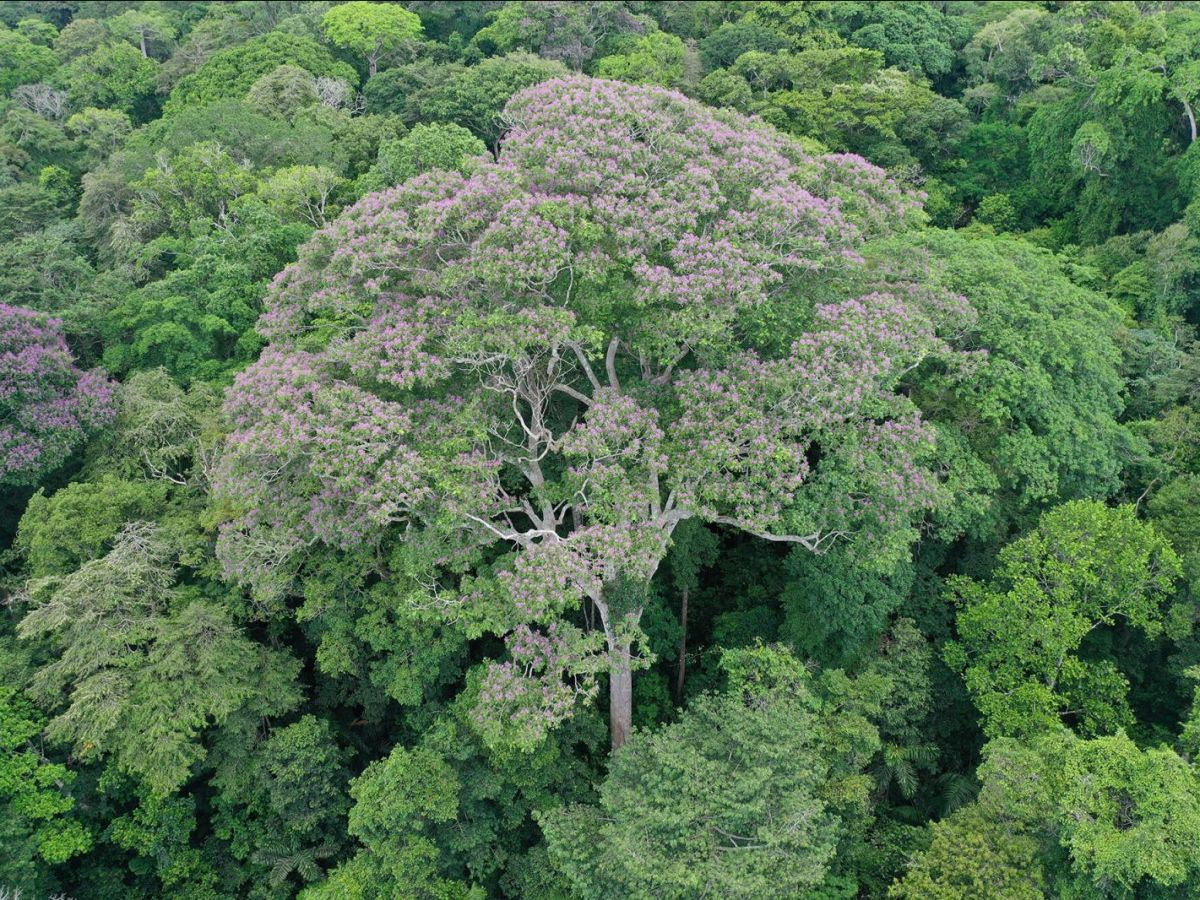
\includegraphics[width=0.49\linewidth]{Pictures/arbre_foudre.jpg}
    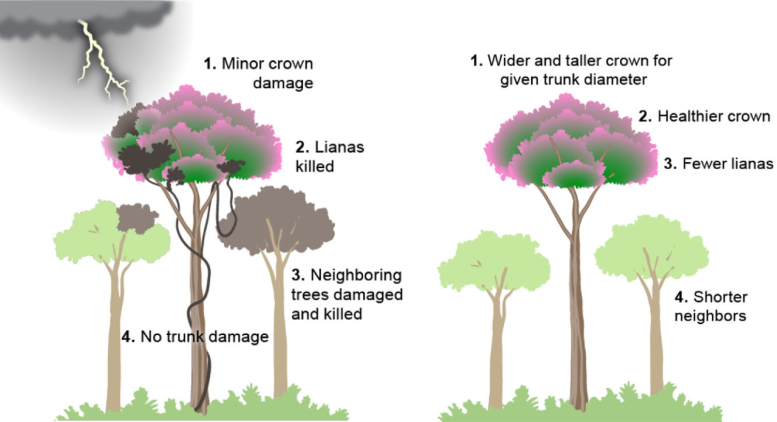
\includegraphics[width=\linewidth]{Pictures/lianes.png}
    \caption{\textbf{En haut à gauche :} Effet de pointe autour d'un arbre. Les équipotentielles sont représentées, ainsi que le champ électrique qui est perpendiculaire aux équipotentielles et d'autant plus important que celles-ci sont resserrées. \textbf{En haut à droite :} photo d'un arbre à fèves Tonka. \textbf{En bas :} observations faites par les scientifiques. Les arbres à fève Tonka sont plus hauts, et attirent la foudre qui les débarrasse de leurs voisins et des lianes. }
    \label{fig:effet_pointe}
\end{figure}

\section{Dipôle électrostatique}

Dans la nature, les charges électriques isolées sont très rares. La force électrostatique est très puissante et a tendance à rassembler les charges de signe opposées pour créer des ensembles neutres à l'échelle macroscopique. C'est le cas notamment des atomes, et plus généralement des molécules.

Le cas le plus simple que l'on puisse imaginer est celui du dipôle électrostatique : un ensemble de deux charges ponctuelles de signe opposé ($+q$ et $-q$) séparées par une distance $a$. En raison de la symétrie du problème, on se place dans un système de coordonnées sphériques en orientant l'axe $(Oz)$ autour du dipôle.

\subsection{Champ créé par un dipôle électrostatique}

Dans cette partie, nous allons nous intéresser au champ créé par un dipôle électrostatique. Pour cela, nous allons raisonner en termes de potentiel électrostatique : en effet, le potentiel $V$ est une grandeur scalaire alors que le champ $\vv E$ est vectoriel. On minimise donc les calculs en utilisant le potentiel $V$ (même si cela reste assez calculatoire...).

\paragraph{Potentiel électrostatique créé par un dipôle}

\begin{figure}[htbp]
    \centering
    % 3D axis with spherical coordinates
\tdplotsetmaincoords{60}{110}
\begin{tikzpicture}[scale=1.5,tdplot_main_coords]
 
  % variables
  \def\rvec{4.5}
  \def\thetavec{42}
  \def\phivec{60}
 
  % axes
  \coordinate (O) at (0,0,0);
  \draw[thick,->] (-0.5,0,0) -- (3,0,0) node[anchor=north east]{$x$};
  \draw[thick,->] (0,-0.5,0) -- (0,3,0) node[anchor=north west]{$y$};
  \draw[thick,->] (0,0,-2) -- (0,0,3) node[anchor=south]{$z$};
 
  % vectors
  \tdplotsetcoord{M}{\rvec}{\thetavec}{\phivec}
  \tdplotsetcoord{Mr}{5.2}{\thetavec}{\phivec}
  \tdplotsetcoord{Mt}{\rvec}{49}{\phivec}
  \tdplotsetcoord{Mp}{\rvec}{\thetavec}{70}
  \draw[thick] (O)  -- (M) node[midway,anchor=east]{$r$};
  \draw[thick,dashed] (0,0,0.75)  -- (M) node[midway,anchor=south]{$r_+$};
  \draw[thick,dashed] (0,0,-0.75)  -- (M) node[midway,anchor=north]{$\,\,r_-$};
  \draw[dashed]   (O)  -- (Mxy);
  \draw[dashed]   (M)  -- (Mxy);
  \draw[dashed]   (My) -- (Mxy);
  \draw[thick,->] (M) -- (Mr) node[anchor=south]{$\vv{e_r}$};
  \draw[thick,->] (M) -- (Mt) node[anchor=west]{$\vv{e_\theta}$};
  \draw[thick,->] (M) -- (Mp) node[anchor=west]{$\vv{e_\varphi}$};

  \filldraw[black] (O) circle (2pt) node[anchor=south east]{$O$};
  \filldraw[black] (M) circle (2pt) node[anchor=south east]{$M$};
  \filldraw[black] (Mxy) circle (2pt) node[anchor=north west]{$H$};
  \filldraw[black] (0,0,.75) circle (2pt) node[anchor=south east]{$+q$};
  \filldraw[black] (0,0,-.75) circle (2pt) node[anchor=north east]{$-q$};
\draw[<->]   (0,-1,-.75)  -- (0,-1,.75) node[midway,anchor=east]{$a$};
\draw[dashed,thick]   (0,-1,.75)  -- (0,0,.75);
\draw[dashed,thick]   (0,-1,-.75)  -- (0,0,-.75);
 
  % arcs
  \tdplotdrawarc[->]{(O)}{2.4}{0}{\phivec}
    {anchor=north}{$\,\,\,\varphi$}
  \tdplotsetthetaplanecoords{\phivec}
  \tdplotdrawarc[->,tdplot_rotated_coords]{(0,0,0)}{1.5}{0}{\thetavec}
    {anchor=south}{$\,\theta$}
 
\end{tikzpicture} \hspace{0.1\textwidth} \begin{tikzpicture}[scale=1.3]
 
  % axes
  \coordinate (O) at (0,0);
  \coordinate (M) at (2.25,2.5);
  \coordinate (H) at (2.25,0);
  \coordinate (Qp) at (0,0.75);
  \coordinate (Qm) at (0,-0.75);
  \draw[thick,->] (0,-2) -- (0,3) node[anchor=south]{$z$};
 
  % vectors

  \filldraw[black] (O) circle (2pt) node[anchor=south east]{$O$};
  \filldraw[black] (M) circle (2pt) node[anchor=south east]{$M$};
  \filldraw[black] (H) circle (2pt) node[anchor=west]{$H$};
  \filldraw[black] (Qp) circle (2pt) node[anchor=south east]{$+q$};
  \filldraw[black] (Qm) circle (2pt) node[anchor=north east]{$-q$};

  \draw[thick,dashed] (Qp) -- (M) node[midway,anchor=east]{$r_+$};
  \draw[thick,dashed] (Qm) -- (M) node[midway,anchor=west]{$r_-$};
  \draw[thick] (O) -- (M) node[midway,anchor=east]{$r$};
  \draw[thick] (H) -- (M) node[midway,anchor=west]{$z$};
  \draw[thick] (H) -- (O) node[midway,anchor=north]{$h$};
  \draw[<->]   (-0.5,0.75)  -- (-0.5,0) node[midway,anchor=east]{$\frac{a}{2}$};
  \draw[<->]   (-0.5,-0.75)  -- (-0.5,0) node[midway,anchor=east]{$\frac{a}{2}$};
\draw[dashed,thick]   (-.5,.75)  -- (Qp);
\draw[dashed,thick]   (-.5,-.75)  -- (Qm);
 
\end{tikzpicture}



\caption{Le dipôle électrostatique est composé de deux charges $+q$ et $-q$. On utilise un système de coordonnées sphériques pour étudier le problème. Figure de gauche : dipôle et système de coordonnées. Figure de droite : représentation dans le plan $(OMH)$.}
\end{figure}


Le potentiel électrostatique généré par le dipôle est donné par la somme des potentiels créés par chacune des deux charges, en vertu du principe de superposition :
\begin{equation}
    V = \frac{q}{4 \pi \varepsilon_0} \left( \frac{1}{r_+} -  \frac{1}{r_-} \right)
\end{equation}
Or en utilisant le schéma de droite on remarque que :
\begin{equation}
    h^2 = r^2 - z^2 = r_+^2 - \left(z-\frac{a}{2}\right)^2
\end{equation}
D'où :
\begin{align}
    r_+^2 &= r^2 +  \left(z-\frac{a}{2}\right)^2 - z^2 \\
    &= r^2 - az + \frac{a^2}{4} \\
    &= r^2 - ar \cos\theta + \frac{a^2}{4} 
\end{align}
où l'on a utilisé $z = r \cos \theta$.

On fera ce que l'on appelle l'approximation dipolaire :
\begin{definition}
    On parle d'approximation dipolaire lorsque l'on étudie le champ créé à une distance grande devant la taille caractéristique du dipôle : $r \gg a$
\end{definition}
Dans ce cas, on peut négliger le dernier terme et on obtient :
\begin{equation}
    r_+^2 \approx r^2 - ar \cos \theta
\end{equation}
Alors en faisant un développement limité à l'ordre 1 :
\begin{equation}
    \frac{1}{r_+} = (r_+^2)^{-\frac{1}{2}} = \frac{1}{r} \left( 1 - \frac{a}{r} \cos \theta\right)^{-\frac{1}{2}} \approx \frac{1}{r} \left( 1 + \frac{a}{2r} \cos \theta \right)
\end{equation}
De même on trouve :
\begin{equation}
    \frac{1}{r_-} \approx \frac{1}{r} \left( 1 - \frac{a}{2r} \cos \theta \right)
\end{equation}
Si bien que l'on obtient au final un potentiel total :
\begin{equation}
    V = \frac{q a \cos \theta}{4 \pi \varepsilon_0 r^2}
\end{equation}

On constate ici que ce potentiel ne dépend que du produit entre la charge portée par les éléments du dipôle et la distance entre ces éléments; on appelle cette quantité le moment dipolaire.


\begin{definition}[Moment dipolaire]
    Soient $M_+$ et $M_-$ deux points portant des charges opposées, respectivement $+q$ et $-q$. On appelle le moment dipolaire électrique de ce dipôle électrostatique la quantité $\vv p = q \vv{M_- M_+}$
\end{definition}

\begin{remark}
    Cette définition coïncide avec la définition vue en chimie avec des charges partielles lorsqu'on a deux charges partielles opposées. Le TD comprend quelques applications d'électrostatique à la chimie (voir notamment l'exercice de solvatation du cuivre). En chimie, on n'a pas forcément une seule charge et dans ce cas, pour un ensemble de charges $q_i$ tel que $\sum q_i = 0$ on définira le moment dipolaire comme $\vv p = \sum q_i \vv{r_i}$ (par exemple pour la molécule d'eau qui comprend une charge $-2\delta$ et deux charges $+\delta$).
\end{remark}

On constate alors que $\theta$ n'est autre que l'angle entre le dipôle électrostatique et le vecteur position, si bien que $a q r \cos \theta = \vv p \cdot \vv r$. Ainsi on obtient une expression générale pour le potentiel électrostatique créé par un dipôle :

\begin{proposition}[Potentiel créé par un dipôle]
    Le potentiel électrostatique créé par un dipôle de moment dipolaire $\vv p$ placé à l'origine $O$ du repère sphérique $(r,\theta,\phi)$ est donné par :
    \begin{equation}
        V = \frac{\vv p \cdot \vv r}{4 \pi \varepsilon_0 r^3}
    \end{equation}
\end{proposition}


\paragraph{Champ électrique créé par un dipôle}

On peut également calculer le champ électrique provoqué par le dipôle. Pour cela, on pourrait réutiliser le principe de superposition mais cette fois-ce sur le champ électrique. Mais il est plus direct d'utiliser la relation $\vv E = - \vv{\mathrm{grad}}(V)$. On utilise en particulier l'expression du gradient en coordonnées sphériques :
\begin{equation}
    \grad = \frac{\partial}{\partial r} \vv{e_r} + \frac{1}{r} \frac{\partial}{\partial \theta}  \vv{e_\theta} + \frac{1}{r \sin \theta} \frac{\partial}{\partial \varphi}  \vv{e_\varphi}
\end{equation}
Ici le potentiel ne dépend que de $\theta$ et de $\phi$ et le champ $\vv E$ est donc donné par :
\begin{align}
    \vv E &= - \grad \left( 
    \frac{q a \cos \theta}{4 \pi \varepsilon_0 r^2} \right) \\
    &= -\frac{qa}{4 \pi \varepsilon_0} \left( \cos \theta \frac{\partial}{\partial r} \left( \frac{1}{r^2} \right) \vv{e_r} + \frac{1}{r^3} \frac{\partial \cos \theta}{\partial \theta} \vv{e_\theta}  \right) \\
    &= \frac{qa}{4 \pi \varepsilon_0 r^3} \left( 2 \cos \theta \, \vv{e_r} + \sin \theta \, \vv{e_\theta}  \right)
\end{align}

\begin{remark}
    L'expression de ce champ n'est pas à connaître par coeur, mais il faut savoir la redémontrer à partir du potentiel, voire même depuis le début (dans ce dernier cas, au concours, la démonstration est souvent guidée par plusieurs questions).
\end{remark}

\paragraph{Equipotentielles et lignes de champ}

Nous pouvons maintenant calculer l'équation des lignes de champ et des équipotentielles, afin de représenter l'allure du champ électrique produit par le dipôle. 

Pour les équipotentielles, il suffit d'écrire que $V$ est constant, ce qui implique que :
\begin{equation}
    \frac{\cos \theta}{r^2} = C
\end{equation}
où $C$ est une constante. Autrement dit, on obtient l'équation polaire des équipotentielles :
\begin{equation}
    r = K \sqrt{|\cos \theta|}
\end{equation}
Elle nous indique que les équipotentielles partent et arrivent en $r=0$ avec un angle $\theta = \pm \pi/2$, et entre les deux tournent en atteignant leur éloignement maximal du dipôle pour $\theta = 0$ ou $\theta = \pi$. Comme la fonction $\sqrt{|\cos \theta|}$ varie très vite lorsque $|\cos \theta|$ est petit, les équipotentielles s'éloignent rapidement du dipôle pour $\theta$ proche de $\pm \pi/2$.


Les lignes de champ sont colinéaires en tout point au champ électrique. Pour calculer l'équation des lignes de champ, nous utilisons l'équivalence entre la colinéarité et un produit vectoriel nul :
\begin{equation}
    \vv E \parallel \vv{\dd \ell} \Leftrightarrow \vv E \wedge \vv{\dd \ell} = \vv 0
\end{equation}
Le champ $\vec E$ n'ayant pas de composante selon $\vv{e_\varphi}$ il en est de même des lignes de champ. En écrivant $\vv{\dd \ell} = \dd r \vv{e_r} + r \dd \theta \vv{e_\theta}$ nous obtenons, après produit vectoriel :
\begin{equation}
    2 r \cos \theta \dd \theta - \sin \theta \dd r = 0
\end{equation}
On utilise une séparation des variables :
\begin{equation}
    \frac{\dd r}{r} = 2 \frac{\dd \theta}{\tan \theta}
\end{equation}
et on obtient après intégration :
\begin{equation}
    \ln r = 2 \ln ( \sin \theta ) + C
\end{equation}
où $C$ est une constante multiplicative. Ceci est équivalent à :
\begin{equation}
    r = K \sin^2 \theta
\end{equation}
où $K$ est une constante multiplicative. On a ainsi l'équation polaire des lignes de champ qui sont des courbes fermées passant par l'origine. Elles partent et arrivent en $r=0$ avec un angle $\theta = 0$ ou $\theta = \pi$, et entre les deux tournent en atteignant leur éloignement maximal du dipôle pour $\theta = \pm \pi/2$. Comme la fonction $\sin^2 \theta}$ varie lentement lorsque $\sin \theta$ est petit, les lignes de champ s'éloignent lentement du dipôle pour $\theta$ proche de 0 ou $\pi$.

\begin{remark}
    Les équations polaires des équipotentielles et des lignes de champ ne sont pas à connaître, mais il est utile de connaître la méthode pour les retrouver.
\end{remark}


On peut maintenant tracer les lignes de champ pour le champ électrique produit par le dipôle, et également en déduire l'allure des équipotentielles qui sont perpendiculaires aux lignes de champ. La formule du potentiel nous indique que celui-ci est positif dans la partie supérieure du plan et négatif dans la partie inférieure.

\begin{figure}[hbtp]
    \centering
    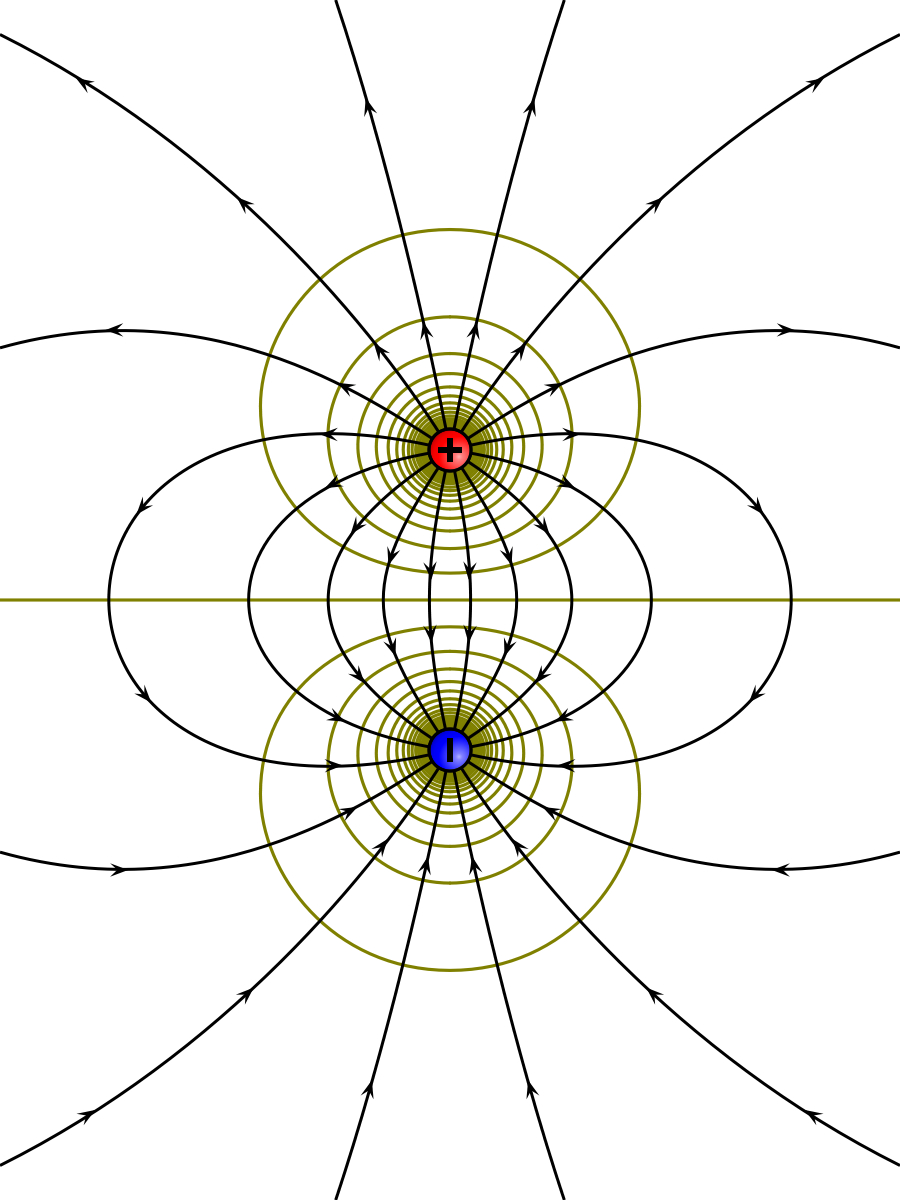
\includegraphics[height=0.45\linewidth]{Pictures/champ_dipole_pres.png} 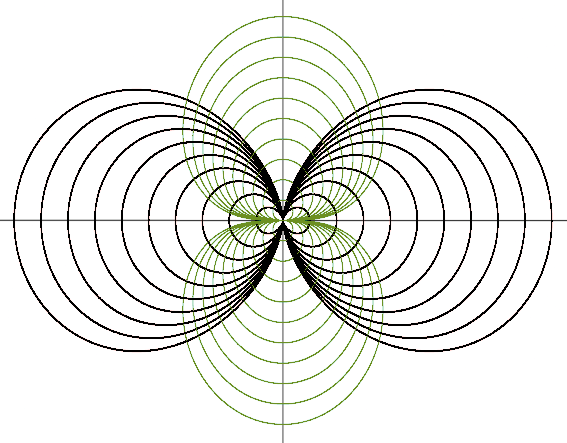
\includegraphics[height=0.45\linewidth]{Pictures/champ_dipole_loin.png}
    \caption{Lignes de champ électrique (en noir) et équipotentielles (en kaki) pour un dipôle électrostatique. La figure de gauche est plus rapprochée du dipôle, et la figure de droite montre ce qui se passe plus loin du dipôle. Dans l'approximation dipolaire (figure de droite), les équations polaires que nous avons établies sont valables. Ceci n'est plus vrai si l'on se rapproche trop du dipôle (figure de gauche). Figures adaptées à partir d'images issues de Wikimedia Commons.}
\end{figure}

\begin{remark}
    L'allure des lignes de champ et équipotentielles créées par un dipôle est à connaître par coeur.
\end{remark}

\subsection{Dipôle dans un champ extérieur}

Nous pouvons maintenant nous poser la question de la réponse d'un dipôle électrostatique à un champ électrique extérieur. Dans toute la suite, nous allons supposer que les deux charges sont solidaires l'une de l'autre (elles sont "attachées" de manière rigide). Elles peuvent représenter, par exemple, une molécule d'eau qui a un moment dipolaire donné. Nous supposons à nouveau que les charges $+q$ et $-q$ se trouvent aux points $M_+$ et $M_-$. Le dipôle associé $\vv p = q \vv{M_- M_+}$ se trouve au point $O$.

\begin{figure}[htbp]
\centering
\begin{tikzpicture}[scale=1.3]
 
  % axes
  \coordinate (O) at (0,0);
  \coordinate (Qp) at (0,1);
  \coordinate (Qm) at (0,-1);
 
  % vectors

  \filldraw[black] (O) circle (2pt) node[anchor=east]{$O$};
  \filldraw[black] (Qp) circle (2pt) node[anchor=south east]{$M_+$};
  \filldraw[black] (Qm) circle (2pt) node[anchor=north west]{$M_-$};

  \draw[thick] (Qp) -- (Qm) ;
  \draw[ultra thick,-stealth] (0,-0.5) -- (0,0.5) node[anchor=west]{$\vv p = q \vv{M_- M_+}$};
  
  \draw[thick,->] (Qp) -- (1,2) node[anchor=west]{$\vv F_+$} ;
  \draw[thick,->] (Qm) -- (-1,-2) node[anchor=east]{$\vv F_-$} ;
\draw[thick,->] (-1.8,-0.3) -- (-1.2,0.3) node[anchor=west]{$\vv E$} ;
\end{tikzpicture}
\caption{Dipôle électrostatique soumis à un champ électrique $\vv E$.}
\end{figure}

\paragraph{Cas d'un champ uniforme}

Si un champ $\vv E$ uniforme est appliqué, alors les deux charges sont soumises à des forces égales et opposées :
\begin{equation}
    \vv F = \vv{F_+} + \vv{F_-} = q \vv E + (-q) \vv E = \vv 0
\end{equation}

Et la résultante des forces qui s'applique sur le dipôle est nulle. En revanche, le moment de ces forces par rapport au point $O$ situé au centre du dipôle est non nul :

\begin{equation}
    \vv{\mathcal{M}} = \vv{\mathcal{M}_+} + \vv{\mathcal{M}_-} = \vv{OM_+} \wedge q \vv E + \vv{OM_-} \wedge (-q) \vv E
\end{equation}
Or on a par la relation de Chasles $\vv{OM_+} - \vv{OM_-} = \vv{M_- M_+}$ et en utilisant la définition du moment dipolaire on trouve l'expression suivante pour le moment de la force électrique sur un dipôle :

\begin{proposition}[Moment des forces électriques sur un dipôle]
    Le moment des forces électrostatiques qui s'appliquent sur un dipôle électrostatique de moment dipolaire $\vv p$ situé dans un champ environnant $\vv E$ est donné par :
\begin{equation}
    \vv{\mathcal{M}} = \vv p \wedge \vv E
\end{equation}
\end{proposition}

\begin{remark}
Nous avons calculé le moment par rapport au point $O$ mais en pratique le moment est le même par rapport à n'importe quel point car la somme des forces qui s'appliquent au dipôle est nulle.
\end{remark}

Ce moment est nul lorsque le dipôle est aligné avec le champ, ainsi les dipôles électrostatiques vont avoir tendance à s'aligner dans le sens du champ. Les charges électriques positives vont avoir tendance à se placer dans les zones de faible potentiel électrique, et inversement. 

On peut, enfin, calculer l'énergie potentielle électrostatique du dipôle électrostatique : 
\begin{equation}
    E_p = q V_+ - q V_-
\end{equation}
Dans le cadre de l'approximation dipolaire, la distance entre les deux charges du dipôle est faible devant la taille caractéristique d'évolution du champ électrique, et on peut raisonnablement supposer que
\begin{equation}
    V(M_+) - V(M_-) = \int_{M_-}^{M_+} - \vv E \cdot \vv{\dd \ell} \approx - \vv E \cdot \vv{M_{-} M_{+}} 
\end{equation}
On en déduit alors l'expression suivante pour l'énergie électrostatique d'un dipôle placé dans un champ extérieur :
\begin{proposition}[Energie potentielle du dipôle électrique]
    L'énergie potentielle électrique d'un dipôle électrostatique $\vv p$ placé dans un champ $\vv E$ est donnée par :
    \begin{equation}
        E_p = - \vv p \cdot \vv E
    \end{equation}
\end{proposition}

On constate que le minimum d'énergie potentielle est atteint lorsque le dipôle est aligné dans le sens du champ.


\paragraph{Champ non uniforme}

Dans le cas d'un champ non uniforme, la force subie par les deux charges peut être légèrement différente. Comme la force de Coulomb est conservative, on peut calculer directement cette force en utilisant le fait qu'elle dérive de l'énergie potentielle électrique :
\begin{equation}
    \vv F = - \grad(E_p) = \grad(\vv p \cdot \vv E)
\end{equation}
Comme les dipôles s'alignent spontanément dans le sens du champ ($\vv p \cdot \vv E > 0$), cette force est orientée vers les zones de champ les plus forts. Ainsi les dipôles sont déviés vers les zones de champ fort.

\begin{remark}
    C'est cette force qui est utilisée aujourd'hui pour manipuler des atomes individuels : on crée une zone de champ électrique très fort avec un laser. Les molécules sont alors attirées vers la zone de champ fort et donc piégées au sein du faisceau. On parle de pince optique. Un exercice du TD aborde ce phénomène de manière plus approfondie.
\end{remark}

\section{Description macroscopique des charges}

Les outils décrits précédemment sont très utiles pour décrire les effets des forces électriques à l'échelle microscopique, par exemple dans un atome ou un cristal, ou sur une molécule avec l'exemple du dipôle.

En revanche, à l'échelle macroscopique, un très grand nombre de charges est présent dans l'espace. Lorsque l'on s'intéresse aux effets du champ électrique à notre échelle, plutôt que de décrire le champ électrique comme la somme de champs créés par des champs individuels, on utilise un approche dite \textbf{macroscopique}.

\subsection{Distribution de charges}

En particulier, nous allons nous intéresser à une grandeur analogue à la densité, qui décrit la quantité de masse par unité de volume, mais cette fois-ci pour l'électrostatique. Pour cela, nous travaillons à une échelle intermédiaire, dite mésoscopique et définie comme suit :

\begin{definition}[Volume mésoscopique]
    Un volume mésoscopique (souvent noté $\mathrm{d}\tau$) est un volume qui contient un grand nombre de particules élémentaires $N \gg 1$, mais dont la taille $\ell$ est petite devant la taille caractéristique $L$ du système macroscopique que l'on étudie: $\ell \ll L$. 
\end{definition}

On prend typiquement $\ell \approx 1$\,µm. L'utilisation de l'échelle mésoscopique nous permet d'avoir une description continue de la matière: à cette échelle et aux échelles plus grandes, la présence de particules chargées distinctes n'est pas importante. On peut alors définir la densité volumique de charge $\rho$:

\begin{definition}[Densité volumique de charge]
    La densité volumique de charge, notée $\rho$, indique la charge nette présente par unité de volume en un point de l'espace. Dans un volume mésoscopique $\mathrm{d}\tau$ contenant une charge $\mathrm{d} q$, on aura ainsi:
    \begin{equation}
        \rho = \frac{\mathrm{d} q}{\mathrm{d}\tau}
    \end{equation}
    La densité volumique de charge est un \textbf{champ scalaire}: elle dépend de la position dans l'espace. Elle peut également dépendre de temps.
\end{definition}

\begin{example}
    Considérons le noyau d'un atome de plomb, qui contient $Z = 82$ protons et $N = 126$ neutrons. La charge totale contenue dans l'atome est :
    \begin{equation}
        Q = Z e
    \end{equation}
    Par ailleurs, le rayon d'un nucléon est d'environ $r_n = 1.2$\,fm (1\,fm\,$=10^{-15}m$). Ceci implique que le volume total du noyau est donné par :
    \begin{equation}
        V = (Z+N) \times \frac{4}{3} \pi r_0^3
    \end{equation}
    On peut supposer que les protons et neutrons sont relativement bien mélangés dans le noyau, et comme $N+Z \gg 1$, on peut également supposer que le noyau est grand devant la taille des nucléons. On peut donc décrire ce noyau par une distribution continue de charges, constituée d'une sphère uniformément chargée avec une densité volumique de charges :
    \begin{equation}
        \rho = \frac{Q}{V} \approx 10^{25} \,\mathrm{C} \cdot \mathrm{m}^{-3}
    \end{equation}
\end{example}

\begin{remark}
    Dans la plupart des solides et solutions aqueuses autour de nous, la densité volumique de charges est nulle: les charges positives et négatives s'équilibrent à l'échelle de l'atome qui est bien plus petite que l'échelle mésoscopique. Ainsi, en général, la description de seuls quelques objets chargés macroscopiquement suffit à bien décrire le champ électrique.
\end{remark}

On peut retrouver la charge totale d'une distribution de charges simplement en intégrant la densité volumique de charges :
\begin{proposition}[Charge totale d'une distribution volumique]
    La charge totale d'une distribution de densité volumique de charges $\rho$ contenue dans un volume $\mathcal{V}$ s'écrit :
    \begin{equation}
        Q_{tot} = \iiint_{\mathcal{V}} \rho \dd \tau
    \end{equation}
\end{proposition}

\paragraph{Densité surfacique de charges}

Dans les conducteurs, on peut observer une accumulation de charges sur la surface du conducteur. Ceci va nous permettre de définir une densité surfacique de charges $\sigma$ :

\begin{definition}[Densité surfacique de charges]
    La densité surfacique de charges, notée $\sigma$, correspond à la charge contenue par unité de surface en un point d'une surface chargée. Si $\dd S$ est un élément mésoscopique de surface qui porte une charge infinitésimale $\dd q$, alors la densité surfacique de charge est :
    \begin{equation}
        \sigma = \frac{\dd q}{\dd S}
    \end{equation}
\end{definition}

\begin{proposition}[Charge totale d'une distribution surfacique]
    La charge totale d'une distribution de densité surfacique de charges $\sigma$ répartie sur une surface $\mathcal{S}$ s'écrit :
    \begin{equation}
        Q_{tot} = \iint_{\mathcal{S}} \sigma \dd S
    \end{equation}
\end{proposition}

\paragraph{Densité linéique de charges}

Enfin pour décrire certaines situations comme un fil, on peut être amené à utiliser une description simplifiée et à faire intervenir la densité linéique de charges :
\begin{definition}[Densité linéique de charges]
    La densité linéique de charges, notée $\lambda$, correspond à la charge contenue par unité de longueur en un point d'un segment chargé. Si $\dd \ell$ est un élément mésoscopique du segment qui porte une charge infinitésimale $\dd q$, alors la densité linéique de charge est :
    \begin{equation}
        \lambda = \frac{\dd q}{\dd \ell}
    \end{equation}
\end{definition}

\begin{example}
Considérons un fil correspondant à un cylindre de rayon $a$, avec une densité volumique de charges uniforme $\rho$. Pour simplifier le modèle, on peut supposer que le rayon $a$ est petit. Alors on modélise le fil par un fil infiniment fin portant une densité linéique de charge $\lambda$. Par définition de la densité volumique de charges, la quantité de charge le long d'un segment $\dd \ell$ est donnée par :
\begin{equation}
    \dd q = \pi a^2 \dd \ell \times \rho
\end{equation}
On en déduit la densité linéique de charges :
\begin{equation}
    \lambda = \pi a^2 \rho
\end{equation}
\end{example}

\begin{proposition}[Charge totale d'une distribution linéique]
    La charge totale d'une distribution de densité linéique de charges $\lambda$ répartie le long d'un chemin $\mathcal{C}$ s'écrit :
    \begin{equation}
        Q_{tot} = \int_{\mathcal{C}} \lambda \dd \ell
    \end{equation}
\end{proposition}

\subsection{Principe de superposition}

Le principe de superposition, qui était vrai pour des charges ponctuelles, l'est aussi pour des distributions de charges quelconques :
\begin{theorem}[Principe de superposition pour des charges ponctuelles]
    Soient deux distribution de charges $\mathcal{D}_1$ et $\mathcal{D}_2$, produisant respectivement des champs électriques $\vv E_1$ et $\vv E_2$. Le champ électrique produit par l'ensemble des deux distributions $\mathcal{D}_1 \cup \mathcal{D}_2$ est $\vv E_1 + \vv E_2$.
\end{theorem}

Ainsi, lorsqu'on résout un problème électrostatique, on a intérêt à découper la distribution de charges en contributions simples, et on peut ensuite utiliser le principe de superposition pour en déduire des informations sur l'ensemble de la distribution.

\subsection{Principe de Curie}

Nous avons maintenant mis en place des outils qui permettent de décrire une distribution macroscopique de charges, via la densité volumique, surfacique ou linéique de charges.

Pour déduire des informations sur le champ électrique, on peut utiliser les propriétés de symétrie de la distribution de charges, en utilisant le principe de Curie :

\begin{theorem}[Principe de Curie]
    Les effets ont les symétries des causes.
\end{theorem}

\subsubsection{Plans de symétrie et antisymétrie}

Ce principe a des conséquences directes concernant les plans de symétrie et d'antisymétrie de la distribution de charges :

\begin{proposition}[Plan de symétrie de la distribution de charges]
    Un plan de symétrie de la distribution de charges est aussi un plan de symétrie du champ électrique. En particulier, le vecteur champ électrique en tout point de ce plan est contenu dans le plan.
\end{proposition}

\begin{proposition}[Plan d'antisymétrie de la distribution de charges]
    Un plan d'antisymétrie de la distribution de charges est aussi un plan d'antisymétrie du champ électrique. En particulier, le vecteur champ électrique en tout point de ce plan est normal à ce plan.
\end{proposition}

Ces deux propriétés peuvent être facilement comprises à travers les exemples géométriques présentés dans la figure \ref{fig:symetries_thibierge}.

\begin{figure}[htbp]
    \centering
    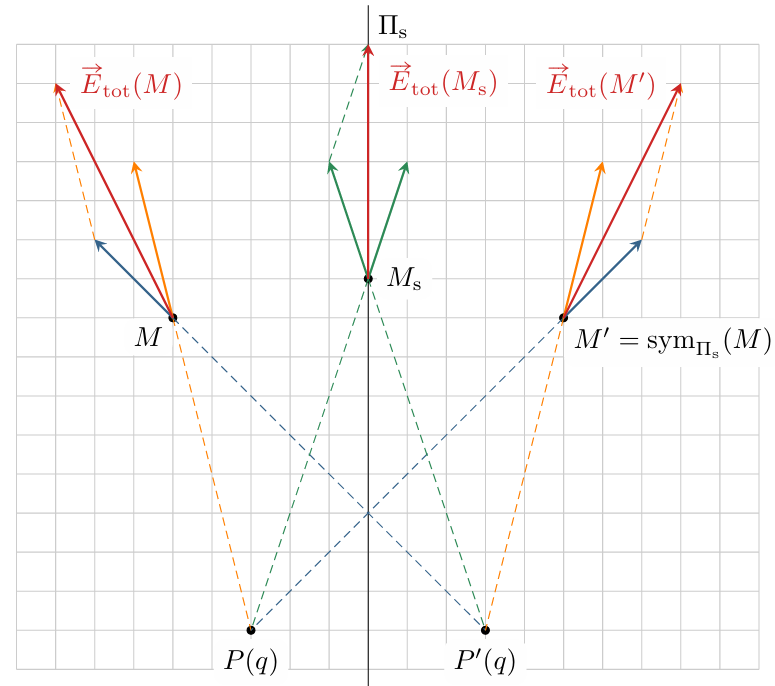
\includegraphics[width=0.49\linewidth]{Pictures/plan_symétrie.png} 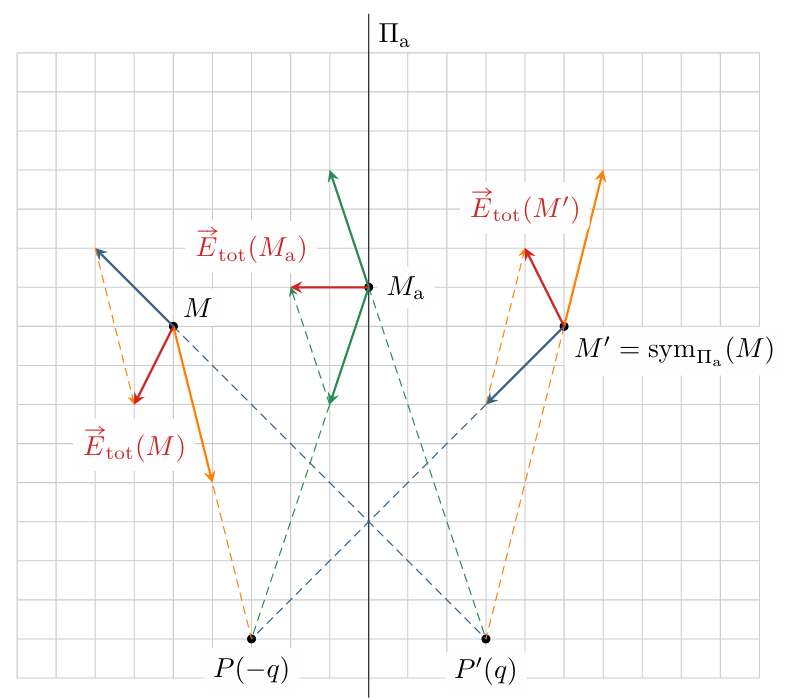
\includegraphics[width=0.49\linewidth]{Pictures/plan_antisymétrie.png}
    \caption{A gauche : Champ électrique produit par deux charges électriques de signe égal situées en $P$ et $P'$, séparées par le plan de symétrie $\Pi_s$. Le plan est aussi un plan de symétrie du champ électrique. En particulier, le vecteur champ électrique en tout point de ce plan est contenu dans le plan. A droite : idem, mais pour des charges de signe opposé. Le plan $\Pi_a$ est maintenant un plan d'antisymétrie. Dans les deux schémas, les vecteurs de même couleur ont même norme, car la norme du champ électrique ne dépend que de la valeur de la charge source $q$ et la distance à la source $r$. Images reproduites du poly de cours d'Etienne Thibierge.}
    \label{fig:symetries_thibierge}
\end{figure}

Nous allons maintenant utiliser ces propriétés pour en déduire des informations sur la direction du champ électrique dans différentes configurations classiques, comme représenté sur la figure \ref{fig:symetries}. Les propriétés issues de l'analyse de la figure \ref{fig:symetries} ne sont pas essentielles à connaître (elles ne sont donc pas encadrées), ce sont plutôt leurs démonstrations qu'il faut savoir refaire. Elles donnent un exemple de la manière dont on peut utiliser les plans de symétrie et d'antisymétrie pour déterminer la direction du champ électrique.

\begin{figure}[htbp]
    \centering
    \tdplotsetmaincoords{60}{110}
\begin{tikzpicture}[scale=0.6,tdplot_main_coords]
 
  % axes
  \draw[thick,->] (0,-2.75,0) -- (0,-2,0);

%Plan arrière
 \draw[thick] (-3,0,3) -- (-3,0,-3) -- (3,0,-3);

%Distrib de charges
\fill[myred!30] (1,-2,-1) -- (1,-2,1) -- (1,2,1) -- (1,2,-1) -- (1,-2,-1);
  \fill[myred!30] (2,-2,0) -- (2,-2,1) -- (2,2,1) -- (2,2,0) -- (2,-2,0);
  \fill[myred!30] (-1,2,-1) -- (-1,2,1) -- (1,2,1) -- (1,2,-1) -- (-1,2,-1);
  \fill[myred!30] (1,2,0) -- (1,2,1) -- (2,2,1) -- (2,2,0) -- (1,2,0);
  \fill[myred!30] (2,2,1) -- (2,-2,1) -- (-1,-2,1) -- (-1,2,1) -- (2,2,1);
  \draw[thick] (-1,-2.,1) -- (-1,2.,1);
  \draw[thick] (2,-2.,1) -- (2,2.,1);
  \draw[thick] (2,-2.,0) -- (2,2.,0);
  \draw[thick] (1,2.,-1) -- (1,-2.,-1);
  \draw[thick,dotted] (-1,2,-1) -- (-1,2,1) -- (2,2,1) -- (2,2,0) -- (1,2,0) -- (1,2,-1) -- (-1,2,-1);

%Plan avant
 \draw[thick] (-3,0,3) -- (3,0,3) -- (3,0,-3) node[anchor=east]{$\Pi_1$};
 \draw[ultra thick,-stealth] (-1.25,0,1.25) -- (-1.75,0,2.5) node[midway,anchor=east]{$\vv E$};

  \draw[thick,->] (0,2,0) -- (0,2.75,0) node[anchor=west]{$z$};

\end{tikzpicture} \begin{tikzpicture}[scale=0.6,tdplot_main_coords]

  %%%%% Cylindre

    % axes
  \draw[thick,->] (0,-2.75,0) -- (0,-2,0);

%Plan arrière
 \draw[thick] (-3,0,3) -- (-3,0,-3) -- (3,0,-3);
 \draw[thick] (3,-2,-3) -- (-3,-2,3) -- (-3,2,3);
 \draw[ultra thick,dashed] (3.5,0,-3.5) -- (-3.5,0,3.5) node[anchor=east]{$\mathcal{D}$};

%Distrib de charges
  \fill[myred!30,canvas is xz plane at y=2] (0,0) circle (1.5);
  \fill[myred!30,canvas is xz plane at y=-2] (0,0) circle (1.5);
\fill[myred!30] (-0.65,-2,1.3) -- (-0.65,2,1.3) -- (0.65,2,-1.3) -- (0.65,-2,-1.3) -- (-0.65,-2,1.3);
  \draw[thick] (-0.65,-2.,1.3) -- (-0.65,2.,1.3);
  \draw[thick] (0.65,2.,-1.3) -- (0.65,-2.,-1.3);
  \draw[thick,dotted,canvas is xz plane at y=2] (0,0) circle (1.5);

%Plan avant
 \draw[thick] (-3,0,3) -- (3,0,3) -- (3,0,-3) node[anchor=south east]{$\Pi_1$};
 \draw[thick] (-3,2,3) -- (3,2,-3) -- (3,-2,-3) node[anchor=east]{$\Pi_2$};
 \draw[ultra thick,-stealth] (-1.25,0,1.25) -- (-2.25,0,2.25) node[midway,anchor=east]{$\vv E$};

  \draw[thick,->] (0,2,0) -- (0,2.75,0) node[anchor=west]{$z$};
 
\end{tikzpicture} \begin{tikzpicture}[scale=0.6,tdplot_main_coords]

  %%%%% Cylindre

    % axes
  \draw[thick] (0,-2.75,0) -- (0,-1,0);

%Plan arrière
 \draw[thick] (-3,0,3) -- (-3,0,-3) -- (3,0,-3);
 \draw[thick] (3,-2,-3) -- (-3,-2,3) -- (-3,2,3);
 \draw[ultra thick,dashed] (3.5,0,-3.5) -- (-3.5,0,3.5) node[anchor=east]{$\mathcal{D}$};

%Distrib de charges
\tdplotsetrotatedcoords{0}{60}{110}
\draw [ball color=myred!30,very thin,tdplot_rotated_coords] (0,0,0) circle (1.5) ;

%Plan avant
 \draw[thick] (-3,0,3) -- (3,0,3) -- (3,0,-3) node[anchor=south east]{$\Pi_1$};
 \draw[thick] (-3,2,3) -- (3,2,-3) -- (3,-2,-3) node[anchor=east]{$\Pi_2$};
 \draw[ultra thick,-stealth] (-1.25,0,1.25) -- (-2.25,0,2.25) node[midway,anchor=east]{$\vv E$};

  \draw[thick,->] (0,1.5,0) -- (0,2.75,0) node[anchor=west]{$z$};
 
\end{tikzpicture} 
\caption{Plans de symétrie de différentes distributions de charges, et conséquences sur la direction du champ électrique. Certains plans de symétrie sont indiqués, en tout point de ces plans le champ électrique est contenu dans le plan. Lorsqu'il y a plusieurs plans de symétrie, le champ électrique $\vv E$ est contenu dans la droite $\mathcal{D}$ à l'intersection des deux plans. Gauche : invariance par translation selon $\vv{e_z}$. Milieu : symétrie cylindrique. Droite : symétrie sphérique.}
\label{fig:symetries}
\end{figure}

\begin{propositionT}[Direction du champ en cas d'invariance par translation]
    Si la distribution de charges est invariante par translation le long d'un axe, alors le champ électrique est en tout point perpendiculaire à cet axe.
\end{propositionT}

\begin{demonstration}
    Cette situation est rencontrée dans les schémas de gauche et du milieu de la figure \ref{fig:symetries}. Nous nous plaçons dans un repère cartésien tel que l'axe d'invariance soit porté par $\vv{e_z}$. Soit $M$ un point quelconque de l'espace, et $\Pi_1$ le plan passant par $M$ et normal à $\vv{e_z}$. Puisque la distribution de charges ne dépend pas de $z$, $\Pi$ est un plan de symétrie de la distribution de charges. Comme $M \in \Pi$, le champ électrique $\vv E(M)$ est contenu dans le plan $\Pi_1$ et donc, par définition du plan $\Pi_1$, est perpendiculaire à $\vv e_z$. Ceci étant vrai pour tout point $M$ on en déduit que le champ électrique est en tout point de l'espace perpendiculaire à $\vv{e_z}$. 
\end{demonstration}

\begin{propositionT}[Direction du champ en cas d'invariance par rotation autour d'un axe]
    Si la distribution de charges est invariante par rotation autour d'un axe $(Oz)$ alors dans le repère cylindrique $(r,\theta,z)$ défini par cet axe, la composante tangentielle du champ électrique est nulle.
\end{propositionT}

\begin{demonstration}
    Cette situation est rencontrée dans les schémas du milieu et de droite de la figure \ref{fig:symetries}. Soit un point $M$ et soit $\Pi_2$ le plan contenant à la fois $M$ et $(Oz)$. Comme la distribution de charges est à symétrie cylindrique autour de $Oz$, $\Pi_2$ est un plan de symétrie de la distribution de charges. Le champ électrique au point $M$ est donc contenu dans ce plan, ce qui implique que la composante tangentielle est nulle. 
\end{demonstration}
\begin{propositionT}[Direction du champ en cas de symétrie sphérique]
    Si la distribution de charges est invariante par rotation autour du point $O$, alors le champ électrique est radial.
\end{propositionT}

\begin{demonstration}
Cette situation est rencontrée dans le schéma de droite de la figure \ref{fig:symetries}. Soit un point $M$ et un plan quelconque passant par $O$ et $M$. Comme la distribution de charges est à symétrie sphérique autour de $O$, ce plan est un plan de symétrie de la distribution de charges. Le champ électrique est donc contenu dans ce plan. Ceci étant vrai pour tout plan contenant $O$ et $M$ (par exemple $\Pi_1$ et $\Pi_2$ sur le schéma), le champ électrique est parallèle à $(OM)$, et donc est orienté selon $\vv{e_r}$.
\end{demonstration}

\subsubsection{Invariances}

Du principe de Curie découle une autre propriété importante, liée aux invariances de la distribution de charges par des translations ou des rotations :

\begin{proposition}[Invariance par translation]
    Si la distribution de charges est invariante par translation le long d'un axe, alors le champ électrique est indépendant de la coordonnée portée par cet axe.
\end{proposition}

\begin{proposition}[Invariance par rotation autour d'un axe]
    Si la distribution de charges est invariante par rotation autour d'un axe $(Oz)$ alors dans le repère cylindrique $(r,\theta,z)$ défini par cet axe, les composantes du champ électrique sont indépendantes de $\theta$.\\
    \textbf{Attention !} Le champ électrique dépend de $\theta$  car les vecteurs $\vv{e_r}$ et $\vv{e_\theta}$ dépendent de $\theta$.
\end{proposition}


\begin{proposition}[Invariance par rotation autour d'un point]
    Si la distribution de charges est invariante par rotation autour d'un point $O$, alors, dans le repère $(r,\theta$,$\phi)$ d'origine $O$, les composantes du champ électrique ne dépendent que de $r$. \\
    \textbf{Attention !} Le champ électrique dépend de $\theta$ et $\phi$ car les vecteur $\vv{e_r}$, $\vv{e_\theta}$ et $\vv{e_\varphi}$ dépendent de $\theta$ et $\phi$.
\end{proposition}

\begin{demonstration}
    Par le principe de Curie, si la distribution de charges est invariante par rotation autour de $O$, les composantes du champ électrique le sont aussi. Elles ne dépendent donc pas de $\theta$ et de $\varphi$ et ne dépendent ainsi que de $r$.
\end{demonstration}

\subsubsection{Forme générale du champ dans des cas de symétrie particuliers} \label{sect:symetries_cas_particuliers}

En combinant les propriétés de symétrie et d'invariance, on obtient la forme générale du champ électrique pour différentes distributions de charges. Il faut être capable de retrouver et de redémontrer ces formes générales.

\begin{propositionT}[Symétrie sphérique]
    Si la distribution de charges est invariante par rotation autour d'un point $O$, alors, dans le repère $(r,\theta$,$\phi)$ d'origine $O$, le champ électrique est de la forme $\vv E = E(r) \vv{e_r}$.
\end{propositionT}

\begin{demonstration}
    Nous avons vu qu'en cas d'invariance par rotation autour d'un point, le champ est radial :
    \begin{equation}
    \vv E = E(r,\theta,\varphi) \vv{e_r}        
    \end{equation}
    Par ailleurs, nous avons aussi vu que ses composantes ne dépendent que de $r$, d'où la forme finale $\vv E = E(r) \vv{e_r}$.
\end{demonstration}

Nous pouvons également étudier la symétrie cylindrique, qui est définie comme suit :

\begin{definition}[Symétrie cylindrique]
    Une distribution de charges est dite à symétrie cylindrique autour d'un ace $(Oz)$ si elle est invariante à la fois par translation le long de cet axe et par rotation autour de cet axe.
\end{definition}

\begin{propositionT}[Symétrie cylindrique]
    Si la distribution de charges est à symétrie cylindrique dans le repère $(r,\theta,z)$ d'axe $(Oz)$ alors le champ électrique est de la forme $\vv E = E(r) \vv{e_r}$
\end{propositionT}

\begin{demonstration}
    Plaçons nous dans le repère $(r,\theta,z)$ d'axe $(Oz)$. La distribution de charges étant invariante par translation de long de $(Oz)$, le champ électrique est indépendant de $z$ et perpendiculaire à $\vv{e_z}$ si bien que :
    \begin{equation}
        \vv E = E_r(r,\theta) \vv{e_r} + E_\theta(r,\theta) \vv{e_\theta}
    \end{equation}
    Or le champ électrique est également invariant par rotation autour de $(Oz)$, il est donc radial, et ses composantes ne dépendent pas de $\theta$. On en déduit :
    \begin{equation}
        \vv E = E(r) \vv{e_r}
    \end{equation}
\end{demonstration}

\begin{encart}[Les symétries : comment faire en pratique ?]
    Il est facile de se perdre dans ces multiples propriétés. Elles sont incluses dans le polycopié pour que vous ayez une vue générale de toutes les situations de symétrie classique.

    \textbf{Comment faire le jour du concours ?} Il est important de citer le principe de Curie et d'utiliser uniquement les propriétés qui en découlent directement, qui sont encadrées dans ce poly :
    \begin{itemize}
        \item Pour identifier la direction du champ, on utilise les propriétés liées aux plans de symétrie et d'antisymétrie ;
        \item Dans le cas d'une invariance par translation, le champ est indépendant de la coordonnée le long de l'axe correspondant;
        \item Dans le cas d'une invariance par rotation, les \textbf{composantes} du champ sont indépendantes de la/des coordonnée(s) angulaire(s) caractérisant cette rotation.
    \end{itemize}
    Il ne faut pas utiliser les propriétés qui ne sont pas encadrées : elles sont présentes dans ce polycopié surtout pour que vous sachiez comment les démontrer.

\textbf{Exemple} Supposons qu'un exercice demande d'établir la forme du champ pour un fil infini chargé. Nous nous plaçons dans le système de coordonnées cylindriques $(r,\theta,z)$ tel que l'axe $(Oz)$ coïncide avec le fil. Soit $M$ un point quelconque de l'espace.

1) Symétries : considérons le plan $\Pi_1$ passant par $M$ et perpendiculaire à $(Oz)$. Ce plan est un plan de symétrie de la distributions de charges. Par le principe de Curie, ce plan est également un plan de symétrie du champ électrique, et donc en tout point de ce plan le champ $\vv E$ est contenu dans ce plan. En particulier, $\vv E(M)$ est contenu dans ce plan et donc $\vv E \cdot \vv{e_z} = 0$. Considérons maintenant le plan $\Pi_2$ passant par $M$ et contenant l'axe $(Oz)$. Ce plan est également un plan de symétrie de la distribution de charges, et donc de la même manière $\vv E(M)$ est contenu dans ce plan. On en déduit $\vv E \cdot \vv{e_\theta} = 0$. On en déduit que le champ est de la forme :
\begin{equation}
    \vv E = E(r,\theta,z) \vv{e_r} 
\end{equation}
    
2) Invariances : la distribution de charges est invariante par translation selon $\vv{e_z}$. Ainsi, par le principe de Curie, le champ $\vv E$ ne dépend pas de $z$. De même, la distribution de charges est invariante par rotation autour de $(Oz)$, donc les composantes du champ $\vv E$ ne dépendent pas de $\theta$. On en déduit que $E(r,\theta,z) = E(r)$.

Conclusion : le champ est de la forme :
\begin{equation}
    \vv E = E(r) \vv{e_r} 
\end{equation}

\end{encart}

\section{Flux du champ électrique}

Une fois les symétries du problème analysées, nous sommes capables de déterminer la forme générale du champ électrique. Nous souhaitons maintenant déterminer précisément le champ électrique créé par une distribution continue de charges. Pour cela, nous allons utiliser le concept du flux d'un vecteur à travers une surface.

\subsection{Flux d'un champ de vecteurs à travers une surface}

Ce concept de flux a déjà été vu en première année, pour un champ uniforme $\vv A$ traversant une surface plane $S$ qui lui est perpendiculaire, le flux du vecteur $\vv A$ à travers cette surface est donné par :
\begin{equation}
    \Phi = \vv A \cdot S \vv n = A S
\end{equation}
où $\vv n$ est la normale par rapport à la surface. 

\begin{figure}[h]
    \centering
    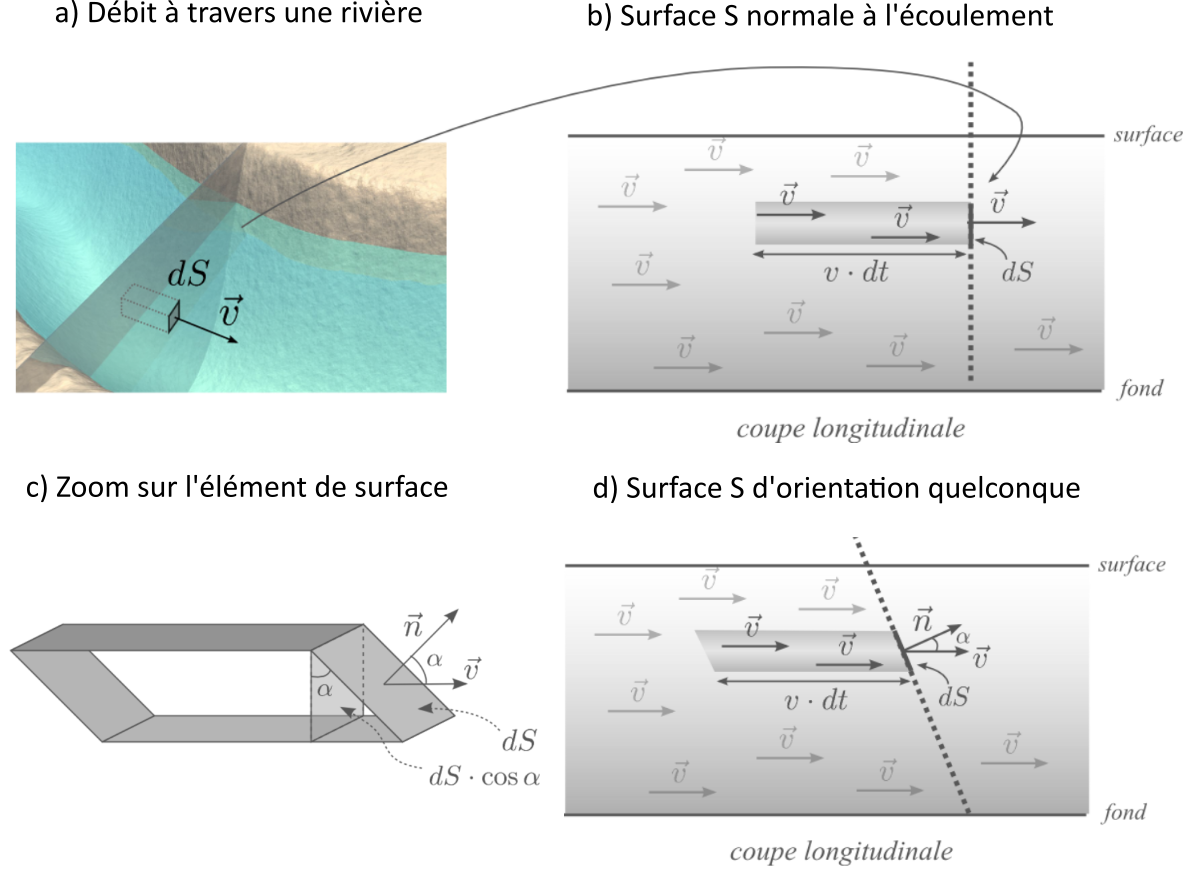
\includegraphics[width=\linewidth]{Pictures/flux_riviere.png}
    \caption{Exemple de calcul d'un flux du champ de vitesses à travers la section d'une rivière pour mesurer un débit (cf encart). a) Schéma général de la situation. b) Situation lorsque la surface est perpendiculaire à l'écoulement. c) et d) situation générale. Les images sont reproduites du poly de cours de Daniel Buskulic.}
    \label{fig:flux_riviere}
\end{figure}

\begin{encart}[Lien entre flux et débit]
La notion de flux se comprend le plus facilement à partir de l'exemple du courant dans une rivière s'écoulant à la vitesse $\vv v$, comme cela est visible sur la figure \ref{fig:flux_riviere}. Dans le cas d'une section plane, le volume d'eau qui traverse une section $\dd S$ perpendiculaire à l'écoulement pendant $\dd t$ est donné par :
\begin{equation}
    \dd V = v \dd t \times \dd S
\end{equation}
Le débit d'eau élémentaire est ainsi donné par :
\begin{equation}
    \dd Q = \frac{\dd V}{\dd t}
 = v \dd S
 \end{equation}
 Intéressons-nous maintenant au cas où la section n'est plus perpendiculaire à l'écoulement mais quelconque. Dans ce cas, comme indiqué sur le schéma de droite, il faut tenir compte de l'angle $\alpha$ entre la vitesse de l'eau et la normale à la surface. Le volume qui traverse la section est maintenant donné par :
 \begin{equation}
    \dd V = v \dd t \times \dd S \times \cos \alpha = \vv v \cdot \vv{\dd S} \dd t
\end{equation}
où l'on a défini un élément de surface orienté selon la normale $\vv n$ à la surface :
\begin{equation}
    \vv{\dd S} = \dd S \vv n
\end{equation}
Le débit total s'obtient par une intégrale sur la surface de tous les débits élémentaires :
\begin{equation}
    Q = \iint_S \dd Q = \iint_S \vv v \cdot \vv{\dd S}
\end{equation}
\end{encart}

Nous allons maintenant élargir ce concept pour une surface non plane et un champ $\vv A$ non uniforme (c'est-à-dire, qui dépend de la position). 

Pour cela, nous découpons la surface en éléments de surface élémentaires, notés $\vv{\dd S}$, qui sont petits devant le rayon de courbure de la surface. Ces éléments de surface sont orientés :

\begin{definition}[Vecteur élément de surface]
    Soit $\mathcal{S}$ une surface, et $\dd S$ un élément de surface petit par rapport à la taille caractéristique de la surface. On note $\vv n$ le vecteur normal à cet élément de surface. Par convention, si la surface est fermée, le vecteur $\vv n$ est pris \textbf{sortant} de la surface.

    On définit alors le vecteur élément de surface :
\begin{equation}
    \vv{\dd S} = \dd S \vv n
\end{equation}
\end{definition}

On peut alors calculer le flux élémentaire du champ $\vv A$ à travers cet élément de surface :
\begin{equation}
    \dd \Phi = \vv A \cdot \vv{\dd S}
\end{equation}

Le flux total est simplement la somme des flux élémentaires à travers chaque élément de surface, ce qui nous amène à la définition suivante :

\begin{definition}[Flux d'un champ de vecteurs]
Soit $\mathcal{S}$ une surface quelconque et $\vv A$ un champ de vecteurs. Le flux du champ $\vv A$ à travers la surface $\mathcal{S}$ est donné par :
\begin{equation}
    \Phi = \iint_{\mathcal{S}} \vv A \cdot \vv{\dd S}
\end{equation}
\end{definition}

\begin{remark}
    Lorsque $\mathcal{S}$ est une surface fermée, on l'indique en plaçant un cercle sur l'intégrale double :
    \begin{equation}
    \Phi = \oiint_{\mathcal{S}} \vv A \cdot \vv{\dd S}
\end{equation}
\end{remark}

\begin{figure}[htbp]
    \centering
    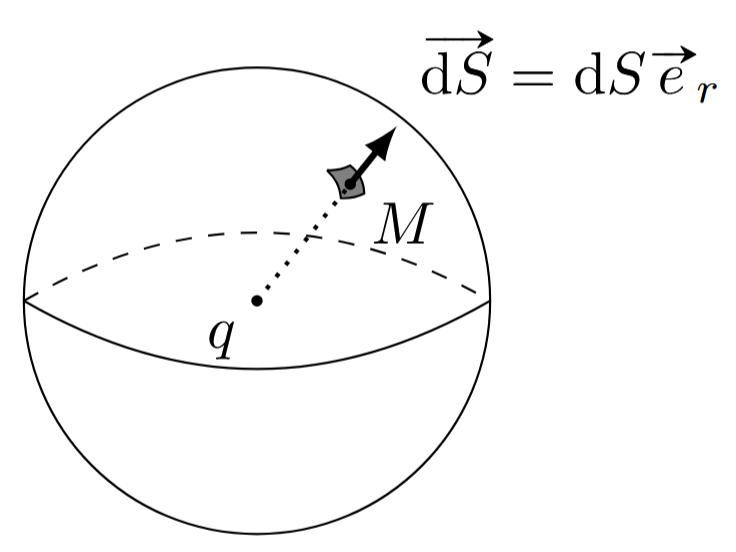
\includegraphics[height=0.35\textwidth]{Pictures/flux_sphere.png} 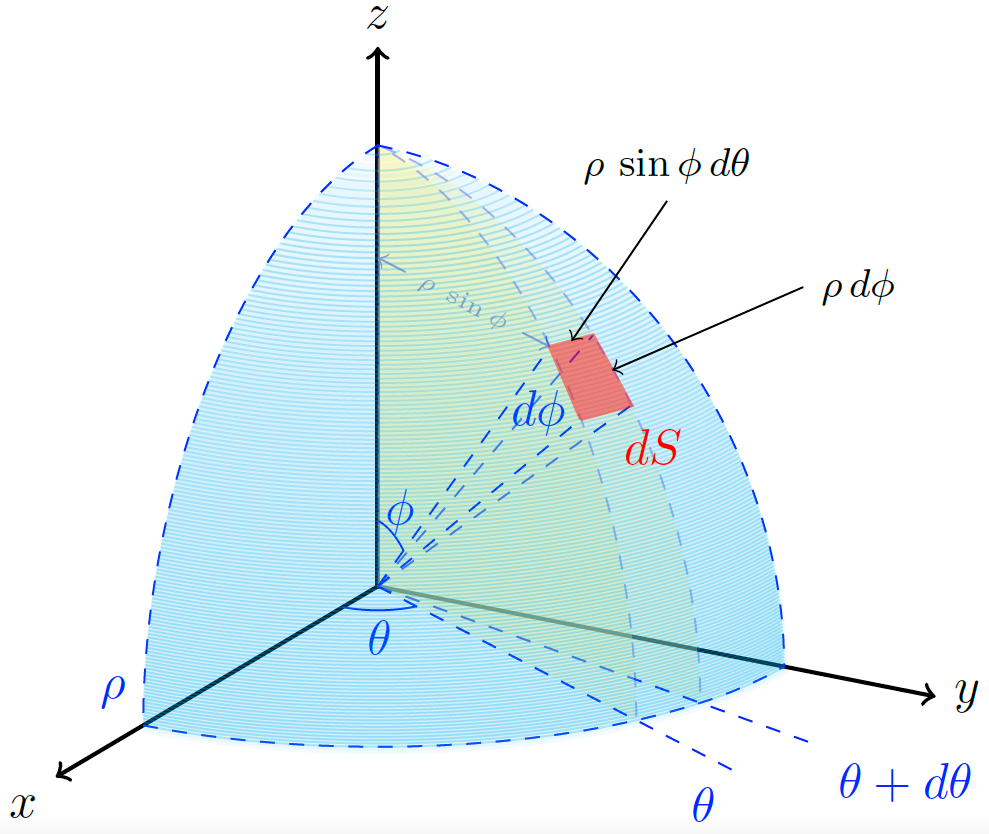
\includegraphics[height=0.35\textwidth]{Pictures/element_de_surface.png}
    \caption{Calcul du flux du champ électrique créé par une charge ponctuelle à travers une sphère. La figure de droite montre le détail du calcul de l'élément de surface. Sources: poly de cours de Maxime Champion et tikz.net .}
    \label{fig:gauss_sphere}
\end{figure}

\begin{example}[Flux du champ électrique créé par une charge ponctuelle à travers une sphère]
    Calculons, par exemple, le flux du champ électrique créé par une charge ponctuelle à travers une sphère centrée sur l'origine.  La situation est représentée sur la figure \ref{fig:gauss_sphere}. Nous nous plaçons dans le système de coordonnées sphériques centré sur l'origine. Si l'élément de surface est pris suffisament petit il est localement plan et assimilable à un parallélépipède rectangle. Sa surface est donnée par :
    \begin{equation}
        \dd S = r \dd \theta \times r \sin \theta \dd \varphi
    \end{equation}
    Par ailleurs, il s'appuie sur le verteur unitaire orthogonal à la surface et sortant, qui n'est autre que $\vv{e_r}$. On en déduit :
    \begin{equation}
        \vv{\dd S} = r^2 \sin \theta \dd \theta  \dd \varphi \vv{e_r}
    \end{equation}

    On peut alors calculer le flux du champ électrique produit par la charge, en remplaçant l'expression de $\vv E$ par celle obtenue via la loi de Coulomb et en utilisant la formule que l'on vient d'obtenir pour $\vv{\dd S}$ :
    \begin{align}
        \Phi &= \oiint_{\mathcal{S}} \vv E \cdot \vv{\dd S} \\
        &= \oiint_{\mathcal{S}} \frac{q}{4 \pi \varepsilon_0 r^2} \vv{e_r} \cdot r^2 \sin \theta \dd \theta \dd \varphi \vv{e_r} \\
        &= \int_{\theta=0}^\pi \int_{\varphi=0}^{2\pi}  \frac{q}{4 \pi \varepsilon_0} \sin \theta \dd \theta \dd \varphi \\
        &= \frac{q}{4 \pi \varepsilon_0} \times 2 \pi \times \int_{\theta=0}^\pi \sin \theta \dd \theta \\
        &= \frac{q}{\varepsilon_0}
    \end{align}

Nous constatons que le flux du champ électrique à travers cette surface est proportionnel à la charge contenue dans la sphère, ce qui n'est pas surprenant : plus la charge est importante et plus le champ électrique qu'elle produit est intense.
    
\end{example}


\subsection{Le théorème de Gauss}

Nous avons vu que le flux du champ électrique autour d'une sphère centrée sur une charge ponctuelle $q$ est donné par :
\begin{equation}
    \Phi = \frac{q}{\varepsilon_0}
\end{equation}
Ce flux est notamment indépendant du rayon choisi pour la sphère.

Cette propriété est remarquable étant donné qu'il n'y a pas de principe physique particulier qui la contraint à être vraie. Nous avons démontré ce résultat uniquement pour une sphère. Mais en réalité, il est valable pour une surface fermée de forme quelconque et pas seulement pour une charge ponctuelle. Il se généralise sous la forme du théorème de Gauss (démonstration complexe et hors programme):

\begin{theorem}[Théorème de Gauss]
    Soit $\mathcal{V}$ un volume contenant une charge électrique $Q_{int}$ et délimité par une surface fermée $\Sigma$. En régime permanent, le flux du champ électrique $\vv E$ à travers la surface $\Sigma$ est donné par :
    \begin{equation}
        \Phi = \oiint_\Sigma \vv E \cdot \vv{\dd S} = \frac{Q_{int}}{\varepsilon_0}
    \end{equation}
\end{theorem}

On constate que le flux du champ électrique à travers une surface fermée ne dépend que des charges contenues à l'intérieur de cette surface. Il s'agit d'une propriété importante du champ électrique.

\subsection{Application aux régions vides de charge}

Si nous appliquons ce théorème dans une région vide de charges, nous constatons que :

\begin{proposition}[Conservativité du flux du champ électrique]
    Dans une région vide de charges, le flux du champ électrique $\vv E$ à travers une surface fermée $\Sigma$ est nul. On dit que le champ $\vv E$ est à flux conservatif.
\end{proposition}

La conservation du flux permet d'obtenir des informations qualitatives sur l'intensité du champ électrique en un point donné. Pour cela, on introduit le concept de tube de champ :

\begin{definition}[Tube de champ]
    Un tube de champ est une surface fermée délimitée par un ensemble de lignes de champ, tronqué par deux sections droites orthogonales.
\end{definition}

\begin{figure}[htbp]
    \centering
    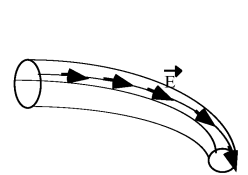
\includegraphics[width=0.3\linewidth]{Pictures/tube_de_champ.png}
    \caption{Tube de champ électrostatique. Source : université de technologie de Compiègne.}
    \label{fig:tube_de_champ}
\end{figure}

Le flux du champ électrique à travers un tube de champ est égal à la somme du flux sortant des deux surfaces orthogonales. En effet, sur le reste de la surface, $\vv E \cdot \vv{\dd S} = 0$ car le vecteur $\vv{\dd S}$ est orthogonal à la surface, qui est elle même colinéaire au champ électrique. On en déduit, en notant $\Sigma_{in}$ et $\Sigma_{out}$ les surfaces par lesquelles le champ électrique entre et sort par le tube de champ, et en appliquant le théorème de Gauss :
\begin{equation}
    \iint_{\Sigma_{in}} \vv E \cdot \vv{\dd S} + \iint_{\Sigma_{out}} \vv E \cdot \vv{\dd S} = 0
\end{equation}
Supposons maintenant que les sections du tube de champ soient prises petites devant les grandeurs caractéristiques du problème. Dans ce cas, on peut considérer que le champ $\vv E$ est uniforme sur chacune de ces surfaces. En notant $S_{in}$ et $S_{out}$ leurs aires respectives, et en se souvenant que le vecteur $\vv{\dd S}$ est orienté vers l'extérieur, on obtient :
\begin{equation}
    ||\vv{E_{in}}|| S_{in} = ||\vv{E_{out}}|| S_{out} = 0
\end{equation}

Autrement dit, plus les lignes de champ électriques se rapprochent, plus la section du tube de champ est faible, et plus le champ électrique est intense. C'est une propriété générale des champs à flux conservatif.

\begin{proposition}[Intensité et lignes de champ]
    Dans un champ à flux conservatif, l'intensité du champ est d'autant plus importante que les lignes de champ sont resserrées.
\end{proposition}


\subsection{Analogie avec la gravitation}

On peut faire une analogie formelle entre l'électrostatique et la théorie de la gravitation, puisque ces deux forces sont des forces centrales, conservatives, et newtoniennes, comme indiqué dans la table \ref{tab:analogie}.

\begin{table}[htbp]
\centering
\begin{tabular}{cc}
\toprule
\textbf{Gravitation} & \textbf{Electrostatique}\\
\midrule
Masse $m$ [kg] & Charge $q$ [C] \\
\midrule
Champ gravitationnel $\vv G$ [m$\cdot$s$^{-2}$] & Champ électrique $\vv E$ [V$\cdot$m$^{-1}$] \\
\midrule
Potentiel gravitationnel $\Phi$ [m$^2\cdot$s$^{-2}$] & Potentiel électrique $V$ [V] \\
\midrule
Force de gravitation & Force de Coulomb \\
$\vv F = \frac{\mathcal{G} m_1 m_2}{r^2} \vv{e_r}$ & $\vv F = \frac{q_1 q_2}{4 \pi \varepsilon_0 r^2} \vv{e_r}$ \\
\midrule
Constante de gravitation universelle $G$ &  $-\frac{1}{4 \pi \varepsilon_0}$ où $\varepsilon_0$ est la permittivité diélectrique du vide  \\
$G = 6,67 \times 10^{-11}$\,m$^3 \cdot$kg$^{-1} \cdot$s$^{-2}$ & $\varepsilon_0 = 8,85 \times 10^{-12}$F$ \cdot$m$^{-1}$ \\
\bottomrule
\end{tabular}
\caption{Analogies entre électrostatique et théorie classique de la gravitation universelle.}
\label{tab:analogie}
\end{table}

Nous avons notamment vu des similarités très fortes entre la structure des lignes de champ et des équipotentielles autour d'une charge ponctuelle ou d'une masse ponctuelle.

Cette analogie formelle nous permet de déduire le théorème de Gauss gravitationnel :
\begin{theorem}[Théorème de Gauss gravitationnel]
    Soit $\mathcal{V}$ un volume contenant une masse électrique $M_{int}$ et délimité par une surface fermée $\Sigma$. Le flux du champ gravitationnel $\vv{\mathcal{G}}$ à travers la surface $\Sigma$ est donné par :
    \begin{equation}
        \Phi = \oiint_\Sigma \vv{\mathcal{G}} \cdot \vv{\dd S} = - 4 \pi G M_{int}
    \end{equation}
\end{theorem}


\begin{remark}
    Une différence fondamentale entre la gravitation est l'électrostatique est que la masse est toujours positive. Il n'existe donc pas d'analogue au dipôle électrostatique en mécanique classique.
    
    En particulier, les lignes de champ gravitationnel convergent toujours vers un objet massique, alors que les lignes de champ électrique peuvent soit converger soit diverger autour d'une charge ponctuelle.
\end{remark}

\section{Deux applications importantes du théorème de Gauss}

\subsection{Sphère uniformément chargée en volume}

Nous allons appliquer le théorème de Gauss et exploiter les symétries d'un problème afin d'établir l'expression du champ électrostatique autour d'une boule uniformément chargée en volume. Considérons une sphère $\mathcal{S}$ de rayon $R$, délimitant un volume $\mathcal{V} = \frac{4}{3} \pi R^3$. Nous supposons que ce volume est chargé uniformément avec une charge totale $Q$. La densité volumique de charge dans le volume est donc donnée par :
\begin{equation}
    \rho = \frac{Q}{\frac{4}{3} \pi R^3}
\end{equation}

\begin{figure}[htbp]
\centering

\begin{tikzpicture}

\filldraw[myred!30] (0,0) circle (1.5) node[anchor=north]{$\rho = \frac{Q}{\frac{4}{3} \pi R^3}$};
\filldraw[black] (0,0) circle (2pt) node[anchor=east]{$O$};
\draw[thick] (0,0) -- (-1.06,1.06) node[midway,anchor=west]{$R$};
\draw[thick] (0,0) -- (2.17,1.25) node[midway,anchor=south]{$r$};
\draw[thick] (0,0) circle (2.5);
\filldraw[black] (1.8,1.8) circle (0pt) node[anchor=south west]{$\mathcal{S}$};
\filldraw[black] (0,-0.3) circle (0pt) node[anchor=north,myred]{$\rho = \frac{Q}{\frac{4}{3} \pi R^3}$};
\end{tikzpicture} \begin{tikzpicture}
\begin{axis}[clip=false,width=7cm,height=5cm,
    axis y line=left, axis x line=bottom,
    xtick={1}, xticklabel = {$R$},
    ytick={1}, yticklabel = {$\frac{Q}{4 \pi \varepsilon_0 R^2}$},
    xmin=0,xmax=3.5,ymin=0,ymax=1.25
    ]
 \addplot[domain=0:1, smooth, samples=3, ultra thick, myred]
    {x}; 
 \addplot[domain=1:3, smooth, samples=25, ultra thick, myred]
    {1/(x^2)}; 
\draw[thick,dashed] (0,1) -- (1,1);
\draw[thick,dashed] (1,0) -- (1,1);
\filldraw[black] (0,1.25) circle (0pt) node[anchor=south]{$E(r)$};
\filldraw[black] (3.5,0) circle (0pt) node[anchor=west]{$r$};
\end{axis}
\end{tikzpicture}

\caption{Modèle de la sphère uniformément chargée en volume.}
\label{fig:enter-label}
\end{figure}

Ce modèle peut correspondre, par exemple, à la description d'un noyau atomique suffisamment gros pour que la répartition des protons et des neutrons dans le noyau puisse être décrite de manière continue. Il faut que le numéro atomique du noyau soit grand devant 1, c'est le cas par exemple de l'atome de plomb ($Z = 82$).

\begin{remark}
    Attention, ce modèle ne correspond pas du tout à la description d'une boule métallique chargée ! En effet, dans un conducteur, les électrons peuvent circuler librement entre les parois et vont circuler jusqu'à annulation totale du champ électrique. Les charges électriques sont donc localisées en surface. On verra cet exemple en TD.
\end{remark}

Nous nous plaçons naturellement dans le système de coordonnées sphériques dont l'origine $O$ coïncide avec le centre de la sphère. 

La distribution de charges est invariante par rotation autour de l'origine $O$. Par le principe de Curie, le champ électrique est radial et sa composante selon $\vv{e_r}$ est invariante par rotation autour de $O$ :
\begin{equation}
    \vv E = E(r) \vv{e_r}
\end{equation}

Nous allons maintenant appliquer le théorème de Gauss. Pour cela, nous choisissons une surface fermée qui va nous permettre d'exploiter la symétrie du problème. Nous prenons une sphère de rayon $r$ centrée sur l'origine. D'après le théorème de Gauss, le flux du champ électrique sortant de la sphère est donné par :
\begin{equation}
    \Phi = \oiint_{\mathcal{S}(r)} \vv E \cdot \vv{\dd S} = \frac{Q_{int}(r)}{\varepsilon_0}
\end{equation}
où $Q_{int}(r)$ est la charge contenue dans la sphère $\mathcal{S}(r)$ de centre $O$ et de rayon $r$.

On distingue alors deux cas de figure :
\begin{itemize}
    \item Si $r > R$ alors $Q_{int} = \frac{4}{3} \pi r^3 \rho = \left( \frac{r}{R} \right)^3 Q$
    \item Si $r>R$ alors $Q_{int} = Q$
\end{itemize}

Par ailleurs, on a $\vv{\dd S} = r^2 \sin \theta \dd \theta \dd \varphi \vv{e_r}$ et l'on peut donc écrire :
\begin{equation}
    \Phi = \int_{\theta=0}^\pi \int_{\varphi=0}^{2\pi} E(r) \vv{e_r} \cdot r^2 \sin \theta \dd \theta \dd \varphi \vv{e_r} = 4 \pi r^2 E(r)
\end{equation}
On obtient donc, en utilisant le théorème de Gauss et l'expression de la charge à l'intérieur de la sphère :
\begin{equation}
    E(r) = \frac{Q r}{4 \pi \varepsilon_0 R^3} \quad \mathrm{si} \quad r<R
\end{equation}
\begin{equation}
    E(r) = \frac{Q}{4 \pi \varepsilon_0 r^2} \quad \mathrm{si} \quad r>R
\end{equation}
Le champ électrique augmente linéairement à l'intérieur de la sphère chargée et est maximal au bord de la sphère, avec une intensité :
\begin{equation}
    || \vv E||_{max} = \frac{Q}{4 \pi \varepsilon_0 R^2}
\end{equation}

A l'extérieur de la sphère, le champ diminue en $1/r^2$. Cette diminution en $1/r^2$ est une conséquence directe de la conservation du flux dans une région vide de charges: elle compense l'augmentation de la surface d'une sphère de rayon $r$, cette surface étant proportionnelle à $r^2$.

\begin{remark}
    On constate que l'expression du champ électrique est identique au champ électrique produit par une charge ponctuelle située au centre de la sphère. Il est remarquable que cette propriété soit valide non seulement loin de la sphère, mais également au voisinage de la sphère. Ceci justifie l'utilisation d'un modèle plus simple pour les noyaux électroniques, dans lequel on les assimile à une charge ponctuelle $+Ze$.
\end{remark}


\subsection{Le condensateur plan}

Nous allons maintenant utiliser le théorème de Gauss pour étudier un dipôle électrique bien connu : le condensateur. Un condensateur est constitué de deux armatures qui sont en influence totale et font partie de conducteurs.

\begin{definition}[Influence totale]
    Deux conducteurs sont dits en influence totale si toutes les lignes de champ qui partent de l'un arrivent sur l'autre, et inversement.
\end{definition}

\begin{proposition}
    Deux conducteurs en influence totale sont porteurs de charges opposées
\end{proposition}

\begin{demonstration}
Par définition de l'influence totale, toutes les lignes de champ partant d'un des deux conducteurs arrivent à l'autre, et vice-versa. Il est donc possible de construire un volume $\mathcal{V}$ formé par l'ensemble des deux conducteurs en influence totale ainsi que par le tube de champ qui est défini par les lignes de champ joignant les deux conducteurs. Puisque toutes les lignes de champ partant d'un conducteur arrivent à l'autre, alors elles sont toutes à l'intérieur du tube de champ. En conséquence, aucune ligne de champ ne sort du volume $\mathcal{V}$ et le flux du champ électrostatique à travers la surface fermée délimitant $\mathcal{V}$ est nul. On en déduit, par le théorèmle de Gauss, que la charge totale contenue dans $\mathcal{V}$ est nulle. Autrement dit, les deux conducteurs sont porteurs de charges opposées.    
\end{demonstration}

Dans un condensateur, les deux conducteurs, typiquement, se font face et sont séparés par un diélectrique. Nous allons considérer le modèle le plus simple de condensateur, constitué de deux armatures planes de taille $L$ séparées par un espace $e$. Nous adoptons le système de coordonnées cartésien, dont l'origine se trouve entre les deux plaques.

En général, l'espace qui sépare les deux armatures est très faible devant la taille des armatures : $e \ll L$. Ceci nous permet de faire l'hypothèse que tout se passe comme si le condensateur était infini dans la direction parallèle aux armatures. 

Nous pouvons donc modéliser notre condensateur par deux plaques infinies, localisées en $z = \pm \frac{e}{2}$, chargées d'une densité surfacique uniforme $\pm \sigma$.

\begin{figure}[htbp]
\centering

\begin{tikzpicture}

\draw[->,thick] (0,-0.5) -- (0,2.5) node[anchor=south]{$z$};

\draw[ultra thick] (1,1) -- (7,1) node[anchor=west]{$-\sigma$};
\draw[ultra thick] (1,2) -- (7,2) node[anchor=west]{$+\sigma$};
\draw[dotted] (0,1) -- (1,1);
\draw[dotted] (0,2) -- (1,2);

\draw[black] (0.2,1) -- (-0.2,1) node[anchor=east]{$-e/2$};
\draw[black] (0.2,2) -- (-0.2,2) node[anchor=east]{$e/2$};


\end{tikzpicture} \hspace{1cm} \begin{tikzpicture}
\draw[thick] (0,1) -- (1.5,1) node[anchor=west]{$-q$};
\draw[thick] (0,1.5) -- (1.5,1.5) node[anchor=west]{$+q$};
\draw[thick] (0.75,0) -- (0.75,0.5);
\draw[thick,->] (0.75,1) -- (0.75,0.5) node[anchor=west]{$i$};
\draw[thick] (0.75,1.5) -- (0.75,2);
\draw[thick,->] (0.75,2.5) -- (0.75,2) node[anchor=west]{$i$};
\draw[thick,->] (-0.5,0.75) -- (-0.5,1.75) node[midway,anchor=east]{$u$};
\filldraw[black] (0,-1) circle (0pt);
\end{tikzpicture}

\caption{Modèles du condensateur plan. A gauche : modèle électrostatique étudié dans ce cours. A droite : modèle simplifié utilisé en électronique.}
\label{fig:condensateur}
\end{figure}


\begin{figure}[htbp]
\centering

\begin{tikzpicture}

\draw[->,thick] (0,-0.5) -- (0,2.5) node[anchor=south]{$z$};

\draw[ultra thick] (1,1) -- (7,1) node[anchor=west]{$\sigma$};
\draw[black] (5,0) -- (5,2) -- (3,2) -- (3,0) -- (5,0) node[anchor=south east]{$\mathcal{S}$};
\draw[dotted] (0,0) -- (3,0);
\draw[dotted] (0,2) -- (3,2);
\draw[dotted] (0,1) -- (1,1);
\draw[dotted] (0,2) -- (1,2);

\draw[black] (0.2,1) -- (-0.2,1) node[anchor=east]{$0$};
\draw[black] (0.2,2) -- (-0.2,2) node[anchor=east]{$z$};
\draw[black] (0.2,0) -- (-0.2,0) node[anchor=east]{$-z$};

\draw[<->] (3,-.3) -- (5,-.3) node[midway,anchor=north]{$H$};
\end{tikzpicture} 

\caption{Etude d'une plaque infinie uniformément chargée en surface.}
\label{fig:surface}
\end{figure}

\paragraph{Plaque uniformément chargée en surface}

Pour commencer, nous allons étudier une seule des deux armatures. Comme indiqué sur la figure \ref{fig:surface} nous supposons l'armature infinie et placée dans le plan $z=0$.

Analysons les symétries du problème :
\begin{itemize}
    \item Le problème est invariant par translation selon $\vv{e_x}$ et $\vv{e_y}$, donc le champ électrique ne dépend que de $z$ : $\vv E = \vv E(z)$.
    \item En tout point $M(x,y,z)$, tout plan passant par $M$ et contenant $\vv{e_z}$ est un plan de symétrie de la distribution de charges, si bien que le champ $\vv E(M)$ est contenu dans tous ces plans et est donc orienté selon $\vv{e_z}$. 
    \item Le plan $z=0$ est un plan de symétrie de la distribution de charges, c'est donc un plan de symétrie du champ électrique, ainsi $\vv E(-z) = -\vv E(z)$
\end{itemize}
On en déduit que :
\begin{equation}
    \vv E = E(z) \vv{e_z}
\end{equation}
et $E(-z) = -E(z)$

Choisissons maintenant une surface de Gauss appropriée. Soit $\mathcal{V}$ le volume délimité par un pavé droit $\mathcal{S}$ dont la base est une surface carrée de taille $H$ dans la dimension horizontale. Le pavé est orienté selon l'axe $\vv{e_z}$ et se trouve entre les altitudes $-z$ et $z$. 

Comme le champ électrique est orienté selon $\vv{e_z}$, cette surface est un tube de champ (quatre des faces du parallélépipède sont colinéaires au champ). Le flux du champ électrique à travers le tube est donné par la différence entre le flux du champ à travers la face supérieure et la face inférieure :
\begin{equation}
    \Phi = \oiint_{\mathcal{S}} \vv E \cdot \vv{\dd S} = H^2 (E(z) - E(-z))
\end{equation}
En utilisant la propriété de symétrie, on obtient :
\begin{equation}
    \Phi = 2 H^2 E(z)
\end{equation}

Par ailleurs, d'après le théorème de Gauss :
\begin{equation}
    \Phi = \frac{Q_{int}(z)}{\varepsilon_0}
\end{equation}
où $Q_{int}(z) = \sigma H^2$ est la charge contenue dans la surface de Gauss. On en déduit que :
\begin{align}
    \vv E(z) &= +\frac{\sigma}{2 \epsilon_0} \vv{e_z} \quad \mathrm{si} \quad z>0\\
    \vv E(z) &= -\frac{\sigma}{2 \epsilon_0} \vv{e_z} \quad \mathrm{si} \quad z<0
\end{align} 

\paragraph{Application au condensateur plan}

Nous revenons au modèle du condensateur plan présenté en figure \ref{fig:condensateur}. Il correspond à une plaque chargée uniformément avec la densité surfacique de charge $+\sigma$, comme étudié précédemment, et une plaque chargée uniformément avec la densité $-\sigma$ pour laquelle la direction  du champ électrique est inversée. En utilisant le principe de superposition nous obtenons :

\begin{align}
    \vv E(z) &= +\frac{\sigma}{2 \epsilon_0} \vv{e_z} -\frac{\sigma}{2 \epsilon_0} \vv{e_z} \quad \mathrm{si} \quad z<-\frac{e}{2}\\
    \vv E(z) &= -\frac{\sigma}{2 \epsilon_0} \vv{e_z} -\frac{\sigma}{2 \epsilon_0} \vv{e_z} \quad \mathrm{si} \quad -\frac{e}{2}<z<\frac{e}{2}\\
    \vv E(z) &= -\frac{\sigma}{2 \epsilon_0} \vv{e_z} +\frac{\sigma}{2 \epsilon_0} \vv{e_z} \quad \mathrm{si} \quad z>\frac{e}{2}\\
\end{align}

Ou, après simplification :
\begin{align}
    \vv E(z) &= -\frac{\sigma}{\epsilon_0} \vv{e_z} \quad \mathrm{si} \quad |z|<\frac{e}{2}\\
    \vv E(z) &= \vv 0 \quad \mathrm{sinon}
\end{align}

Le champ électrique est donc nul à l'extérieur du condensateur, et le champ électrique est uniquement présent entre les deux armatures.

\paragraph{Lien avec les propriétés macroscopiques du condensateur}

Il est possible maintenant de revenir à notre modèle du condensateur et d'utiliser ces résultats pour étudier le comportement du condensateur à l'échelle macroscopique. En particulier, nous allons démontrer la loi reliant courant et tension aux bornes d'un condensateur, qui a été admise en première année.

Pour cela, on calcule la tension aux bornes du condensateur, qui n'est autre que la différence de potentiel entre les armatures. La différence de potentiel est donnée par la circulation du champ le long d'une ligne qui relie les armatures :
\begin{equation}
    u = - \int_{-\frac{e}{2}}^{\frac{e}{2}} \vv E \cdot \dd z \vec{e_z} = \frac{\sigma e}{\varepsilon_0}
\end{equation}
Autrement dit, le potentiel électrique est maximal sur l'armature chargée positivement.

Par ailleurs, si $S$ est la surface des armatures (que l'on a supposée telle que $\sqrt{S} \gg e$), la charge totale portée par les armatures est $q = \sigma S$.

Ainsi, il est possible de relier la charge portée par les armatures à la tension entre ces armatures via la relation :
\begin{equation}
    q = C u
\end{equation}
et l'on obtient la capacité du condensateur plan :
\begin{proposition}
    La capacité d'un condensateur plan, dont les armatures ont une surface $S$ et sont séparées par une distance $e$, est donnée par :
    \begin{equation}
        C = \frac{\varepsilon_0 S}{e}
    \end{equation}
\end{proposition}

On peut remarquer que si l'on dérive temporellement la relation $q = C u$. En effet, le courant qui pénètre dans l'armature de charge positive correspond à la variation de charge de cette armature :
\begin{equation}
    i = \frac{\dd q}{\dd t}
\end{equation}
si bien que
\begin{equation}
    i = C \frac{\dd u}{\dd t}
\end{equation}
et l'on retrouve l'expression bien connue du lien entre tension et intensité aux bornes d'un condensateur.


\end{document}

\section{Applications à l'échelle mésoscopique}

Afin de traduire cette propriété de manière microscopique, nous allons introduire un nouvel outil mathématique : la divergence.


\begin{definition}[Divergence]
    Soit un volume mésoscopique $\mathrm{d}\tau$ centré sur un point $P$ délimité par une surface fermée $\mathrm{d}S$. La divergence d'un champ $\vv A$ au point $P$ est définie de façon à ce que le flux élémentaire $\delta \Phi$ du champ $\vv A$ à travers la durface $\mathrm{d}S$ soit donné par :
    \begin{equation}
        \delta \Phi = \mathrm{div}(\vv A) \mathrm{d}S
    \end{equation}
\end{definition}

\begin{proposition}[Divergence en coordonnées cartésiennes]
    En coordonnées cartésiennes, la divergence d'un champ $\vv A$ s'écrit :
    \begin{equation}
        \mathrm{div}(\vv A) = \frac{\partial A_x}{\partial x} + \frac{\partial A_y}{\partial y} + \frac{\partial A_z}{\partial z}
    \end{equation}
\end{proposition}

\begin{demonstration}
Considérons un volume $\mathrm{d}\tau = \mathrm{d}x \mathrm{d}y \mathrm{d}z$ situé entre les plans $x$ et $x+\mathrm{d}x$, $y$ et $y+\mathrm{d}y$, $z$ et $z+\mathrm{d}z$. Le flux du champ $\vv A$ sortant à travers les surfaces délimitant le volume $\mathrm{d}\tau$ et normales à $\vv{e_x}$ est donné par :
\begin{equation}
    \delta \Phi_x = A_x(x+\dd x) \dd y \dd z - A_x(x) \dd y \dd z = \frac{\partial A_x}{\partial x} \dd x \dd y \dd z
\end{equation}
Les flux élémentaires $\delta \Phi_y$ et $\delta \Phi_z$ à travers les surfaces normales à $\vv{e_y}$ et $\vv{e_z}$ se calculent de la même manière et on obtient finalement :
\begin{equation}
    \delta \Phi = \delta \Phi_x + \delta \Phi_y + \delta \Phi_z = \left( \frac{\partial A_x}{\partial x} + \frac{\partial A_y}{\partial y} + \frac{\partial A_z}{\partial z} \right) \dd \tau
\end{equation}
Or par définition de la divergence :
 \begin{equation}
        \delta \Phi = \mathrm{div}(\vv A) \mathrm{d}S
\end{equation}
On en déduit :
\begin{equation}
        \mathrm{div}(\vv A) = \frac{\partial A_x}{\partial x} + \frac{\partial A_y}{\partial y} + \frac{\partial A_z}{\partial z}
\end{equation}
\end{demonstration}

On peut également calculer la divergence en coordonnées cartésiennes ou sphériques. Elle est donné dans le formulaire.


\subsection{Équation de Maxwell-Gauss}

Nous avons vu plus haut que dans le cas d'une unique charge ponctuelle, le flux du champ électrique à travers une sphère centrée sur une charge $q$ est donné par : $\Phi = q/\varepsilon_0$. 

Cette propriété se généralise à une distribution de charges quelconque via une équation établie à l'échelle microscopique : c'est l'équation de Maxwell-Gauss.

\begin{theorem}[\'{E}quation de Maxwell-Gauss]
    Soit une distribution de charges $\rho(\vv r)$. Cette distribution produit un champ électrique $\vv E$ tel que :
    \begin{equation}
        \mathrm{div}(\vv E) = \frac{\rho}{\varepsilon_0}
    \end{equation}
\end{theorem}

Cette équation est un postulat qui a été fait notamment à partir des observations de Coulomb concernant la décroissance de la force électroqtatique en $1/r^2$. Néanmoins, il est possible de comprendre d'où elle vient.

Soit maintenant un volume sphérique mésoscopique $\dd \tau$ délimité par une surface $\dd S$, et contenant une charge $\dd q$. Par principe de superposition, le flux du champ électrique à travers la surface $\dd S$ est donné par la somme des flux $\delta \Phi_i$ causés par toutes les charges élémentaires $q_i$ de la distribution de charges :
\begin{equation}
    \delta \Phi = \sum_{i} \delta \Phi_i
\end{equation}
Si la charge $q_i$ est située dans la sphère, on a $\delta \Phi = \frac{q_i}{\varepsilon_0}$. En revanche, si elle est en dehors de la sphère, on a $\delta \Phi = 0$. Ainsi on obtient une somme sur les charges qui sont contenues dans le volume $\dd \tau$:
\begin{equation}
    \delta \Phi = \sum_{i \in \dd \tau} \frac{q_i}{\varepsilon_0}
\end{equation}
Autrement dit, puisque la somme des charges élémentaires dans le volume $\dd \tau$ n'est autre que $\dd q$ :
\begin{equation}
    \delta \Phi = \frac{\dd q}{\varepsilon_0}
\end{equation}
Or, par définition de la divergence :
\begin{equation}
    \delta \Phi = \mathrm{div}(\vv E) \dd \tau
\end{equation}
Et par définition de la densité volumique de charges :
\begin{equation}
    \dd q = \rho \dd \tau
\end{equation}
Si bien que l'on obtient :
\begin{equation}
    \mathrm{div}(\vv E) = \frac{\rho}{\varepsilon_0}
\end{equation}


L'équation de Maxwell-Gauss est utile pour décrire le comportement du champ électrique à l'échelle microscopique, mais elle peut également être utilisée à l'échelle macroscopique. Pour cela, on utilise le théorème de Green-Ostrogradski :

\begin{theorem}[Théorème de Green-Ostrogradski]
    Soit $\vv A$ un champ vectoriel, $V$ un volume et $\Sigma$ la surface fermée délimitant ce volume. Alors la divergence du champ $\vv A$ dans le volume $V$ est reliée au flux du champ $\vv A$ à travers la surface $\Sigma$ par la relation suivante :
    \begin{equation}
        \iiint_V \mathrm{div}(\vv A) \dd \tau = \oiint_\Sigma \vv A \cdot \vv{\dd S}
    \end{equation}
\end{theorem}

\begin{remark}
    Le cercle sur la seconde intégrale indique qu'elle est réalisée sur une surface fermée.
\end{remark}

\begin{demonstration}
    (pour un volume cubique) On se concentre sur un volume cubique délimité par $x \in [0,X]$, $y \in [0,Y]$, $z \in [0,Z]$. Le flux du champ $\vv A$ à travers la surface délimitant ce volume est donné par la somme des flux à travers les six faces du cube, que l'on peut décomposer selon les directions $\vv{e_x}$, $\vv{e_y}$ et $\vv{e_z}$. En particulier :
\begin{equation}
    \Phi_x = \int_{y=0}^Y \int_{z=0}^Z A_x(X,y,z) \dd z \dd y - \int_{y=0}^Y \int_{z=0}^Z A_x(0,y,z) \dd z \dd y
\end{equation}
Par ailleurs, en utilisant la forme cartésienne de la divergence ($\mathrm{div} \vv A = \partial_x A_x + \partial_y A_y + \partial_z A_z$ on peut décomposer l'intégrale volumique de la divergence en trois composantes, dont la première s'écrit :
\begin{align}
    \iiint_V \frac{\partial A_x}{\partial x} \dd \tau &= \int_{z=0}^Z \int_{y=0}^Y \left( \int_{x=0}^X \frac{\partial A_x}{\partial x} \dd x \right) \dd y \dd z \\
    &= \int_{z=0}^Z \int_{y=0}^Y (A_x(X,y,z) - A_x(0,y,z)) \dd y \dd z
\end{align}
On reconnaît que les composantes sont égales. Il en est de même pour les composantes selon $y$ et $z$. Ainsi, pour un volume cubique, le théorème de Green-Ostrogradski est vérifié.
\end{demonstration} 

On admettra que ce théorème est valide pour un volume de taille quelconque.


\end{document}


Il est par ailleurs possible (mais hors programme) de montrer que flux du champ électrique produit par une charge ponctuelle est inchangé si la charge ne se trouve pas au centre de la sphère. Enfin, on peut aussi montrer que le flux du champ électrique généré par une charge se trouvant à l'extérieur de la sphère est nul.  

\begin{figure}[htbp]
\centering
\tdplotsetmaincoords{60}{110}
\begin{tikzpicture}[scale=1,tdplot_main_coords]
 \coordinate (O) at (0,0,0);
\filldraw[black] (O) circle (2pt) node[anchor=north]{$q$};
\filldraw[black] (0,0,-3) circle (0pt) node[anchor=north]{$\Phi = 0$};
\path[tdplot_screen_coords,ball color=myred!30,opacity=0.5] (O) circle[radius=2]; 

\end{tikzpicture}
\begin{tikzpicture}[scale=1,tdplot_main_coords]
 \coordinate (O) at (0,0,0);
\filldraw[black] (0,1,-1) circle (2pt) node[anchor=north]{$q$};
\filldraw[black] (0,0,-3) circle (0pt) node[anchor=north]{$\Phi = \frac{q}{\varepsilon_0}$};
\path[tdplot_screen_coords,ball color=myred!30,opacity=0.5] (O) circle[radius=2]; 
\end{tikzpicture}
\begin{tikzpicture}[scale=1,tdplot_main_coords]
 \coordinate (O) at (0,0,0);
\filldraw[black] (0,1.7,-1.7) circle (2pt) node[anchor=north]{$q$};
\filldraw[black] (0,0,-3) circle (0pt) node[anchor=north]{$\Phi = 0$};
\path[tdplot_screen_coords,ball color=myred!30,opacity=0.5] (O) circle[radius=2]; 
\end{tikzpicture}
\caption{Le flux du champ électrique produit par une charge ponctuelle à travers des sphères centrées ou non sur la charge.}
\end{figure}


\begin{figure}[htbp]
\centering
\tdplotsetmaincoords{60}{110}
\begin{tikzpicture}[scale=1,tdplot_main_coords]
 \coordinate (O) at (0,0,0);
\filldraw[black] (0,1.7,-1.7) circle (2pt) node[anchor=north]{$q_1$};
\filldraw[black] (0,1.,-1.6) circle (2pt) node[anchor=north]{$q_2$};
\filldraw[black] (0,-2.8,-0.5) circle (2pt) node[anchor=north]{$q_3$};
\filldraw[black] (0,-1.3,-0.5) circle (2pt) node[anchor=north]{$q_4$};
\filldraw[black] (0,1.3,1.1) circle (2pt) node[anchor=north]{$q_5$};
\filldraw[black] (0,0.1,-0.1) circle (2pt) node[anchor=north]{$q_6$};
\filldraw[black] (0,-1,.9) circle (2pt) node[anchor=north]{$q_7$};
\path[tdplot_screen_coords,ball color=myred!30,opacity=0.5] (O) circle[radius=2]; 
\end{tikzpicture}
\caption{Situation plus complexe avec une distribution de charges composée de plusieurs charges ponctuelles.}
\end{figure}

Considérons maintenant une sphère quelconque, et supposons que l'espace est occupé par des charges $q_i$ localisées aux poins $M_i$. Nous notons $\vv{r_i} = \vv{M_i P}$ où $P$ est le point courant. Par principe de superposition, le champ électrique en tout point $P$ est donné par :
\begin{equation}
    \vv E = \sum_i \frac{q_i}{4 \pi \varepsilon_0 \vv{r_i}^3} \vv{r_i} 
\end{equation}
Et le flux de ce champ à travers la sphère $\mathcal{S}$ s'écrit :
\begin{equation}
    \Phi = \sum_i \Phi_i = \sum_i \oiint_{\mathcal{S}}  \frac{q_i}{4 \pi \varepsilon_0 \vv{r_i}^3} \vv{r_i} \cdot \vv{\dd S}
\end{equation}

Nous pouvons maintenant séparer les charges qui appartiennent au volume $\mathcal{V}$ délimité par la sphère et celles qui ne lui appartiennent pas :
\begin{equation}
    \Phi = \sum_{i | M_i \in \mathcal{V}} \Phi_i + \sum_{i | M_i \notin \mathcal{V}} \Phi_i
\end{equation}
Or, nous avons vu que le flux $\Phi_i$ est égal à $\frac{q_i}{\varepsilon_0}$ si $M_i \in \mathcal{V}$ et est nul sinon. Nous pouvons donc en déduire que :
`\begin{equation}
    \Phi = \sum_{i | M_i \in \mathcal{V}} \frac{q_i}{\varepsilon_0}
\end{equation}
en notant $Q_{int} = \sum_{i | M_i \in \mathcal{V}} q_i$ la charge totale contenue dans la sphère, on obtient finalement une relation entre le flux du champ électrique à travers la sphère et la charge totale contenue dans cette sphère :
\begin{equation}
    \Phi = \frac{Q_{int}}{\varepsilon_0}
\end{equation}

\paragraph{Circularité des lignes de champ (FAUX)}

Il est possible de montrer que ces lignes de champ sont des cercles :
\begin{proposition}[Lignes de champ du dipôle électrostatique]
    Dans le cadre de l'approximation dipolaire, les lignes de champ électrique créées par un dipôle $\vv p$ sont des cercles tangents à $\vv p$.
\end{proposition}

\begin{figure}[htbp]
    \centering
    
\begin{tikzpicture}[scale=1.3]
 
  % axes
  \coordinate (O) at (0,0);
  \coordinate (K) at (4,0);
  \coordinate (C) at (2,0);
  \coordinate (M) at (3.414,1.414);
  \coordinate (Mx) at (3.414,0);
  \coordinate (My) at (0,1.414);
  \draw[thick,->] (0,-2.25) -- (0,2.25) node[anchor=south]{$z$};
  \draw[thick,->] (-0.5,0) -- (5,0);
  \draw[ultra thick,-] (4,0.15) -- (4,-0.15) node[anchor=north]{$\,\,K$};
  \draw[ultra thick,-] (2,0.15) -- (2,-0.15) node[anchor=north]{$\frac{K}{2}$};
 
  % vectors

  \filldraw[black] (O) circle (2pt) node[anchor=north east]{$O$};
  \filldraw[black] (M) circle (2pt) node[anchor=south west]{$M$};
  \filldraw[black] (C) circle (2pt) node[anchor=south east]{$O'$};

  \draw[thick] (K) arc (0:360:2) ;
  \draw[thick,->] (0,0.5) arc (270:203:-0.5) node[midway,anchor=south]{$\theta$} ;
  \draw[thick,dotted] (C) -- (2,0.5) ;
  \draw[thick,->] (2,0.5) arc (270:225:-0.5) node[midway,anchor=south]{$\beta$} ;

  
  \draw[thick,dotted] (M) -- (My) node[anchor=east]{$r \cos \theta$};
  \draw[thick,dotted] (M) -- (Mx) node[anchor=north]{$r \sin \theta$};

  
  \draw[ultra thick,-stealth] (0,-0.7) -- (0,0.7) node[anchor=east]{$\vv p$};
  

  \draw[thick] (C) -- (M) node[midway,anchor=west]{$\rho$};
  \draw[thick] (O) -- (M) node[midway,anchor=south]{$r$};
 
\end{tikzpicture}

    \caption{Schéma d'une ligne de champ et variables utilisées pour démontrer que cette ligne de champ est circulaire. On cherche à montrer que la variable $\rho$ est une constante.}
\end{figure}

\begin{demonstration}

Nous souhaitons montrer que ces lignes de champ, d'équation $r = K \sin \theta$, sont des cercles.  Puisque la distance à l'origine le long d'une ligne de champ varie entre $0$ et $K$, on peut raisonnablement supposer que ces cercles sont de rayon $K/2$, et nous notons $O'$ le centre présumé du cercle, de coordonnées $r=K/2$ et $\theta = \pi/2$. Notre objectif est de montrer que la distance $\rho$ entre un point quelconque de la ligne de champ $M$ et le point $O'$ est constante. 


Pour le vérifier, nous considérons l'une de ces lignes de champ. Nous avons alors, avec les angles définis sur le schéma :
\begin{equation}
    r \sin \theta = \frac{K}{2} + \rho \sin \beta 
\end{equation}
\begin{equation}
    r \cos \theta = \rho \cos \beta 
\end{equation}
En éliminant $\beta$ via la relation $\cos^2 \beta + \sin^2 \beta = 1$ nous obtenons :
\begin{equation}
    \rho^2 = \left( r \sin \theta - \frac{K}{2} \right)^2 + (r \cos \theta)^2 = r^2 + \left( \frac{K}{2} \right)^2 - r K \sin \theta
\end{equation}
Nous pouvons alors remplacer par l'expression de $r$ en coordonnées polaires $r = K \sin \theta$ pour trouver :
\begin{equation}
    \rho^2 = \left( \frac{K}{2} \right)^2
\end{equation}
Autrement dit, $\rho$ est constant, et les lignes de champ sont bien des cercles tangents au dipôle électrostatique.
    
\end{demonstration}



%----------------------------------------------------------------------------------------
%	PART
%----------------------------------------------------------------------------------------

\part{Part One}

%----------------------------------------------------------------------------------------
%	CHAPTER 1
%----------------------------------------------------------------------------------------

\chapterimage{chapter_head_2.pdf} % Chapter heading image

\chapter{Text Chapter}

\section{Paragraphs of Text}\index{Paragraphs of Text}

\lipsum[1-7] % Dummy text

%------------------------------------------------

\section{Citation}\index{Citation}

This statement requires citation \cite{book_key}; this one is more specific \cite[122]{article_key}.

%------------------------------------------------

\section{Lists}\index{Lists}

Lists are useful to present information in a concise and/or ordered way\footnote{Footnote example...}.

\subsection{Numbered List}\index{Lists!Numbered List}

\begin{enumerate}
\item The first item
\item The second item
\item The third item
\end{enumerate}

\subsection{Bullet Points}\index{Lists!Bullet Points}

\begin{itemize}
\item The first item
\item The second item
\item The third item
\end{itemize}

\subsection{Descriptions and Definitions}\index{Lists!Descriptions and Definitions}

\begin{description}
\item[Name] Description
\item[Word] Definition
\item[Comment] Elaboration
\end{description}

%----------------------------------------------------------------------------------------
%	CHAPTER 2
%----------------------------------------------------------------------------------------

\chapter{In-text Elements}

\section{Theorems}\index{Theorems}

This is an example of theorems.

\subsection{Several equations}\index{Theorems!Several Equations}
This is a theorem consisting of several equations.

\begin{theorem}[Name of the theorem]
In $E=\mathbb{R}^n$ all norms are equivalent. It has the properties:
\begin{align}
& \big| ||\mathbf{x}|| - ||\mathbf{y}|| \big|\leq || \mathbf{x}- \mathbf{y}||\\
&  ||\sum_{i=1}^n\mathbf{x}_i||\leq \sum_{i=1}^n||\mathbf{x}_i||\quad\text{where $n$ is a finite integer}
\end{align}
\end{theorem}

\subsection{Single Line}\index{Theorems!Single Line}
This is a theorem consisting of just one line.

\begin{theorem}
A set $\mathcal{D}(G)$ in dense in $L^2(G)$, $|\cdot|_0$. 
\end{theorem}

%------------------------------------------------

\section{Definitions}\index{Definitions}

This is an example of a definition. A definition could be mathematical or it could define a concept.

\begin{definition}[Definition name]
Given a vector space $E$, a norm on $E$ is an application, denoted $||\cdot||$, $E$ in $\mathbb{R}^+=[0,+\infty[$ such that:
\begin{align}
& ||\mathbf{x}||=0\ \Rightarrow\ \mathbf{x}=\mathbf{0}\\
& ||\lambda \mathbf{x}||=|\lambda|\cdot ||\mathbf{x}||\\
& ||\mathbf{x}+\mathbf{y}||\leq ||\mathbf{x}||+||\mathbf{y}||
\end{align}
\end{definition}

%------------------------------------------------

\section{Notations}\index{Notations}

\begin{notation}
Given an open subset $G$ of $\mathbb{R}^n$, the set of functions $\varphi$ are:
\begin{enumerate}
\item Bounded support $G$;
\item Infinitely differentiable;
\end{enumerate}
a vector space is denoted by $\mathcal{D}(G)$. 
\end{notation}

%------------------------------------------------

\section{Remarks}\index{Remarks}

This is an example of a remark.

\begin{remark}
The concepts presented here are now in conventional employment in mathematics. Vector spaces are taken over the field $\mathbb{K}=\mathbb{R}$, however, established properties are easily extended to $\mathbb{K}=\mathbb{C}$.
\end{remark}

%------------------------------------------------

\section{Corollaries}\index{Corollaries}

This is an example of a corollary.

\begin{corollary}[Corollary name]
The concepts presented here are now in conventional employment in mathematics. Vector spaces are taken over the field $\mathbb{K}=\mathbb{R}$, however, established properties are easily extended to $\mathbb{K}=\mathbb{C}$.
\end{corollary}

%------------------------------------------------

\section{Propositions}\index{Propositions}

This is an example of propositions.

\subsection{Several equations}\index{Propositions!Several Equations}

\begin{proposition}[Proposition name]
It has the properties:
\begin{align}
& \big| ||\mathbf{x}|| - ||\mathbf{y}|| \big|\leq || \mathbf{x}- \mathbf{y}||\\
&  ||\sum_{i=1}^n\mathbf{x}_i||\leq \sum_{i=1}^n||\mathbf{x}_i||\quad\text{where $n$ is a finite integer}
\end{align}
\end{proposition}

\subsection{Single Line}\index{Propositions!Single Line}

\begin{proposition} 
Let $f,g\in L^2(G)$; if $\forall \varphi\in\mathcal{D}(G)$, $(f,\varphi)_0=(g,\varphi)_0$ then $f = g$. 
\end{proposition}

%------------------------------------------------

\section{Examples}\index{Examples}

This is an example of examples.

\subsection{Equation and Text}\index{Examples!Equation and Text}

\begin{example}
Let $G=\{x\in\mathbb{R}^2:|x|<3\}$ and denoted by: $x^0=(1,1)$; consider the function:
\begin{equation}
f(x)=\left\{\begin{aligned} & \mathrm{e}^{|x|} & & \text{si $|x-x^0|\leq 1/2$}\\
& 0 & & \text{si $|x-x^0|> 1/2$}\end{aligned}\right.
\end{equation}
The function $f$ has bounded support, we can take $A=\{x\in\mathbb{R}^2:|x-x^0|\leq 1/2+\epsilon\}$ for all $\epsilon\in\intoo{0}{5/2-\sqrt{2}}$.
\end{example}

\subsection{Paragraph of Text}\index{Examples!Paragraph of Text}

\begin{example}[Example name]
\lipsum[2]
\end{example}

%------------------------------------------------

\section{Exercises}\index{Exercises}

This is an example of an exercise.

\begin{exercise}
This is a good place to ask a question to test learning progress or further cement ideas into students' minds.
\end{exercise}

%------------------------------------------------

\section{Problems}\index{Problems}

\begin{problem}
What is the average airspeed velocity of an unladen swallow?
\end{problem}

%------------------------------------------------

\section{Vocabulary}\index{Vocabulary}

Define a word to improve a students' vocabulary.

\begin{vocabulary}[Word]
Definition of word.
\end{vocabulary}

%----------------------------------------------------------------------------------------
%	PART
%----------------------------------------------------------------------------------------

\part{Part Two}

%----------------------------------------------------------------------------------------
%	CHAPTER 3
%----------------------------------------------------------------------------------------

\chapterimage{chapter_head_1.pdf} % Chapter heading image

\chapter{Presenting Information}

\section{Table}\index{Table}

\begin{table}[h]
\centering
\begin{tabular}{l l l}
\toprule
\textbf{Treatments} & \textbf{Response 1} & \textbf{Response 2}\\
\midrule
Treatment 1 & 0.0003262 & 0.562 \\
Treatment 2 & 0.0015681 & 0.910 \\
Treatment 3 & 0.0009271 & 0.296 \\
\bottomrule
\end{tabular}
\caption{Table caption}
\end{table}

%------------------------------------------------

\section{Figure}\index{Figure}

\begin{figure}[h]
\centering
\includegraphics[scale=0.5]{placeholder}
\caption{Figure caption}
\end{figure}

%----------------------------------------------------------------------------------------
%	BIBLIOGRAPHY
%----------------------------------------------------------------------------------------

\chapter*{Bibliography}
\addcontentsline{toc}{chapter}{\textcolor{ocre}{Bibliography}}
\section*{Books}
\addcontentsline{toc}{section}{Books}
\printbibliography[heading=bibempty,type=book]
\section*{Articles}
\addcontentsline{toc}{section}{Articles}
\printbibliography[heading=bibempty,type=article]

%----------------------------------------------------------------------------------------
%	INDEX
%----------------------------------------------------------------------------------------

\cleardoublepage
\phantomsection
\setlength{\columnsep}{0.75cm}
\addcontentsline{toc}{chapter}{\textcolor{ocre}{Index}}
\printindex

%----------------------------------------------------------------------------------------
